%%%%%%%%%%%%%%%%%%%%%%%%%%%%%%%%%%%%%%%%%
% This is a template for LaTeX thesis (M.Sc. or PhD) at ZHAW.
% 
% ZHAW thesis template downloaded from:
% https://github.com/matteodelucchi/ZHAW_thesis-template
% 
% University specific changes were made by:
% Matteo Delucchi
%
% Based on a template downloaded from:
% http://www.LaTeXTemplates.com
% 
% Version 2.x major modifications by:
% Vel (vel@latextemplates.com)
%
% This template is based on a template by:
% Steve Gunn (http://users.ecs.soton.ac.uk/srg/softwaretools/document/templates/)
% Sunil Patel (http://www.sunilpatel.co.uk/thesis-template/)
%
% Template license:
% CC BY-NC-SA 3.0 (http://creativecommons.org/licenses/by-nc-sa/3.0/)
%
%%%%%%%%%%%%%%%%%%%%%%%%%%%%%%%%%%%%%%%%%

%----------------------------------------------------------------------------------------
%	PACKAGES AND OTHER DOCUMENT CONFIGURATIONS
%----------------------------------------------------------------------------------------

\documentclass[
11pt, % The default document font size, options: 10pt, 11pt, 12pt
%oneside, % Two side (alternating margins) for binding by default, uncomment to switch to one side
spanish, % ngerman for German
singlespacing, % Single line spacing, alternatives: onehalfspacing or doublespacing
%draft, % Uncomment to enable draft mode (no pictures, no links, overfull hboxes indicated)
%nolistspacing, % If the document is onehalfspacing or doublespacing, uncomment this to set spacing in lists to single
%liststotoc, % Uncomment to add the list of figures/tables/etc to the table of contents
%toctotoc, % Uncomment to add the main table of contents to the table of contents
%parskip, % Uncomment to add space between paragraphs
%nohyperref, % Uncomment to not load the hyperref package
headsepline, % Uncomment to get a line under the header
%chapterinoneline, % Uncomment to place the chapter title next to the number on one line
%consistentlayout, % Uncomment to change the layout of the declaration, abstract and acknowledgements pages to match the default layout
]{MastersDoctoralThesis} % The class file specifying the document structure

\usepackage[utf8]{inputenc} % Required for inputting international characters
\usepackage[T1]{fontenc} % Output font encoding for international characters
\usepackage{xcolor}

%\usepackage[x-5pg]{pdfx} %for PDF-X support. Has problems with xcolor and hyperref
%\usepackage{subfigure}
\usepackage{caption}
\usepackage{subcaption}

\usepackage{mathpazo} % Use the Palatino font by default

\usepackage[backend=biber,  % Use the bibtex backend with the authoryear citation style (which resembles APA)
sorting=none, % numbers the reference in order of their appearance in the document. Troubleshoot with deleting all *.aux and *.bbl files and rebuild.
style=numeric-comp,
natbib=true]{biblatex}

\addbibresource{example.bib} % The filename of the bibliography

\usepackage[autostyle=true]{csquotes} % Required to generate language-dependent quotes in the bibliography

\usepackage{pdfpages}

\usepackage{todonotes}
\setlength{\marginparwidth}{2.5cm} % uncomment this if the todonotes are out of margins (cut off page)

\usepackage{listings}

\usepackage[acronym]{glossaries}



\definecolor{codegreen}{rgb}{0,0.6,0}
\definecolor{codegray}{rgb}{0.5,0.5,0.5}
\definecolor{codepurple}{rgb}{0.58,0,0.82}
\definecolor{backcolour}{rgb}{0.921, 0.929, 0.937} %0.95,0.95,0.92

\lstdefinestyle{mystyle}{
backgroundcolor=\color{backcolour},   
commentstyle=\color{codegreen},
keywordstyle=\color{magenta},
numberstyle=\tiny\color{codegray},
stringstyle=\color{codepurple},
basicstyle=\ttfamily\footnotesize,
breakatwhitespace=false,         
breaklines=true,                 
captionpos=b,                    
keepspaces=true,                 
numbers=left,                    
numbersep=5pt,                  
showspaces=false,                
showstringspaces=false,
showtabs=false,                  
tabsize=2
}

\lstset{style=mystyle}

\usepackage{makecell} % formatting tables





%----------------------------------------------------------------------------------------
%	MARGIN SETTINGS
%----------------------------------------------------------------------------------------

\geometry{
paper=a4paper, % Change to letterpaper for US letter
inner=2.5cm, % Inner margin
outer=3.8cm, % Outer margin
bindingoffset=.5cm, % Binding offset
top=1.5cm, % Top margin
bottom=1.5cm, % Bottom margin
%showframe, % Uncomment to show how the type block is set on the page
}


%----------------------------------------------------------------------------------------
%	THESIS INFORMATION
%----------------------------------------------------------------------------------------

\thesistitle{Seguridad en redes neuronales artificiales: Vulnerabilidades y contramedidas} % Your thesis title, this is used in the title and abstract, print it elsewhere with \ttitle
\supervisor{Dr. Fernando Berzal Galiano} % Your supervisor's name, this is used in the title page, print it elsewhere with \supname
\examiner{} % Your examiner's name, this is not currently used anywhere in the template, print it elsewhere with \examname
\degree{Máster Ingeniería Informática} % Your degree name (Doctor of Philosophy or Master of Science), this is used in the title page and abstract, print it elsewhere with \degreename
\author{Rodrigo Orellana Flores} % Your name, this is used in the title page and abstract, print it elsewhere with \authorname
\addresses{} % Your address, this is not currently used anywhere in the template, print it elsewhere with \addressname

\subject{} % Your subject area, this is not currently used anywhere in the template, print it elsewhere with \subjectname
\keywords{} % Keywords for your thesis, this is not currently used anywhere in the template, print it elsewhere with \keywordnames
\university{\href{https://www.ugr.es}{Universidad de Granada}} % Your university's name and URL, this is used in the title page and abstract, print it elsewhere with \univname
\universitygerman{\href{https://www.ugr.es}{Universidad de Granada}{}}% Your university's name in german and URL, this is used in the german abstract (Zusammenfassung), print it elsewhere with \univnameger
 %department's name and URL, this is used in the title page and abstract, print it elsewhere with \deptname
\group{\href{}{}} % Your research group's name and URL, this is used in the title page, print it elsewhere with \groupname
\faculty{\href{https://etsiit.ugr.es/}{Escuela Técnica Superior de Ingenierías Informática y de
Telecomunicación}} % Your faculty's name and URL, this is used in the title page and abstract, print it elsewhere with \facname

\AtBeginDocument{
\hypersetup{pdftitle=\ttitle} % Set the PDF's title to your title
\hypersetup{pdfauthor=\authorname} % Set the PDF's author to your name
\hypersetup{pdfkeywords=\keywordnames} % Set the PDF's keywords to your keywords
}

%%%%%%%%%%%%%%%%%%%%%%%%%%%% GLOSARIO
\makeglossaries
\newglossaryentry{latex}
{
        name=latex,
        description={Is a mark up language specially suited for scientific documents}
}

\newglossaryentry{maths}
{
        name=mathematics,
        description={Mathematics is what mathematicians do}
}

\newglossaryentry{formula}
{
        name=formula,
        description={A mathematical expression}
}


\begin{document}

\frontmatter % Use roman page numbering style (i, ii, iii, iv...) for the pre-content pages

\pagestyle{plain} % Default to the plain heading style until the thesis style is called for the body content

%----------------------------------------------------------------------------------------
%	TITLE PAGE
%----------------------------------------------------------------------------------------

\begin{titlepage}
\begin{center}

\begin{figure}
\centering

\includegraphics[width=0.4\textwidth]{Figures/ugr3.png} % Universtiy Logo, Adapted from: https://upload.wikimedia.org/wikipedia/commons/thumb/e/e6/ZHAW_Logo.svg/879px-ZHAW_Logo.svg.png
\end{figure}
{\huge \bfseries Universidad de Granada\par}\vspace{0.4cm} % Thesis title
{\normalsize \facname \par}% Faculty name

\vspace*{.06\textheight}


			%{\normalsize \deptname \par}% Department name
			%\bigskip



{\scshape\LARGE TRABAJO FIN DE MÁSTER\par}\vspace{0.5cm}  
\textsc{\Large INGENIERÍA INFORMÁTICA}\\[0.5cm] 

\HRule \\[0.4cm] % Horizontal line
{\huge \bfseries Seguridad en redes neuronales artificiales: Vulnerabilidades y contramedidas\par}\vspace{0.4cm} % Thesis title
\HRule \\[1.5cm] % Horizontal line
 
\begin{minipage}[t]{0.4\textwidth}
\begin{flushleft} \large
\emph{Autor:}\\
\href{https://github.com/rodrigo-orellana}{\authorname} % Author name - remove the \href bracket to remove the link
\end{flushleft}
\end{minipage}
\begin{minipage}[t]{0.4\textwidth}
\begin{flushleft} \large
\emph{Director:} \\
\href{http://elvex.ugr.es/}{\supname} % Supervisor name - remove the \href bracket to remove the link  
\end{flushleft}
\end{minipage}\\[2.5cm]
 
\vfill


%
\includegraphics[width=0.32\textwidth]{Figures/etsiit.jpeg} %logo escuela 
\hspace{1cm}
%
\includegraphics[width=0.35\textwidth]{Figures/decsai.jpg} %logo departamento


%\large \textit{Escuela Técnica Superior de Ingenierías Informática y de Telecomunicación}\\[0.6cm] % University requirement text
%\textit{--}\\[0.6cm]
Departamento de Ciencias de la Computación e Inteligencia Artificial
\\
Granada, septiembre de 2020\\[2cm] % Research group name and department name
 
\vfill

%{\large \today}\\[4cm] % Date
%\includegraphics{Logo} % University/department logo - uncomment to place it
 
\vfill
\end{center}
\end{titlepage}


%\cleardoublepage

%----------------------------------------------------------------------------------------
%	ABSTRACT PAGE
%----------------------------------------------------------------------------------------

\begin{abstract}
\addchaptertocentry{\abstractname}
Las redes de aprendizaje profundo en inteligencia artificial han destacado en la última década con resultados sorprendentes en aplicaciones como visión artificial, conducción automática de vehículos, detección de fraudes bancarios, interpretación de comandos de voz, filtrado de seguridad de redes y otros más,  abriendo paso a una nueva era a nivel tecnológico. Sin embargo, han surgido muchas investigaciones en busca de brindar seguridad en su operación, debido a que se ha descubierto que dichas redes son vulnerables en cuanto a sus resultados entregados cuando una entrada ha sido adulterada de manera imperceptible a una revisión humana. Este ejercicio es llamado ataque adversario, en donde el atacante busca hacer fallar la clasificación o incluso dirigirla a hacia una respuesta deseada. Esto implica un riesgo en la aplicación de esta tecnología que incluso puede suponer riesgos de vidas humanas, economías de países o de la privacidad de las personas. Actualmente este es un incidente abierto, ya que no se ha planteado una solución definitiva para asegurar la robustez de las redes profundas, Sin embargo, han surgido ciertos avances para proteger a los modelos de ciertos tipos de ataques particulares.
El objetivo de este proyecto es en primer lugar realizar un estudio del estado del arte en cuanto a la seguridad de las redes profundas, luego realizar experimentos planteando, ejecutando y analizando resultados de ataques a distintos modelos. Por otro lado, se plantea y experimenta una contramedida que brinda robustez al modelo.


\end{abstract}

%----------------------------------------------------------------------------------------
%	German ABSTRACT PAGE
%----------------------------------------------------------------------------------------


\begin{extraAbstract}
\addchaptertocentry{\extraabstractname} % Add the abstract to the table of contents
Deep learning in artificial intelligence has stood out in the last decade with surprising results on applications such as artificial vision, automatic vehicle driving, bank fraud detection, interpretation of voice commands, network security filtering, and others, paving the way for a new era at the technological level. However, there have been many kinds of research on providing security in their operation, because it has been discovered vulnerabilities on networks in terms of their results when an entry has been crafted imperceptibly for a human review. This issue is called an Adversarial attack, where the attacker tries to fail de system or even direct it towards the desired response. This implies a risk in the application of this technology that can even imply risk on human lives, economic, or the privacy of people. Currently, this is an open incident, since a definitive solution has not been proposed to ensure the robustness of deep networks. However, certain advances have emerged to protect the models from certain types of particular attacks.
The objective of this project is firstly to carry out a study of the state of the art regarding the security of deep networks, then to carry out experiments, executing and analyzing the results of attacks on different models. On the other hand, a defense methodology is proposed and experienced.


    
\end{extraAbstract}
%----------------------------------------------------------------------------------------
%	ACKNOWLEDGEMENTS
%----------------------------------------------------------------------------------------

\begin{acknowledgements}
\addchaptertocentry{\acknowledgementname} % Add the acknowledgements to the table of contents
 A través de estas líneas quiero expresar mi más sincero agradecimiento a todas aquellas personas que a lo largo de mi vida han creído en mí, partiendo por mis padres que me convencieron de que no hay metas suficientemente altas como para no ser alcanzadas.

También agradecer a mi universidad de grado que me dio valores como la autoconfianza, perseverancia, coraje y valentía para enfrentar cualquier desafío profesional.

Por otro lado, al coordinador del máster y a cada uno de los profesores que forman parte del programa, especialmente a Fernando, el director de este trabajo, quien me motivó a desarrollar la temática de este estudio y me guio en el desarrollo de la misma con gran interés, comprensión y carisma. Sin duda fue un acierto solicitar que fuera mi tutor.

También quisiera mencionar a mi compañera de aventuras que me ayudó a sobrepasar los momentos difíciles y me brindó su apoyo incondicional y con quien nunca falta un motivo para celebrar.
\\
\begin{flushright}
Gracias, totales\ldots
\end{flushright} 
\end{acknowledgements}



%----------------------------------------------------------------------------------------
%	LIST OF CONTENTS/FIGURES/TABLES PAGES
%----------------------------------------------------------------------------------------

\tableofcontents % Prints the main table of contents

%\listoffigures % Prints the list of figures

%\listoftables % Prints the list of tables

%----------------------------------------------------------------------------------------
%	ABBREVIATIONS
%----------------------------------------------------------------------------------------







%----------------------------------------------------------------------------------------
%	DEDICATION
%----------------------------------------------------------------------------------------

\dedicatory{Dedicado a mi hija, nunca dejes de buscar tus sueños \ldots} 


%----------------------------------------------------------------------------------------
%	THESIS CONTENT - CHAPTERS
%----------------------------------------------------------------------------------------

\mainmatter % Begin numeric (1,2,3...) page numbering

\pagestyle{thesis} % Return the page headers back to the "thesis" style

% Include the chapters of the thesis as separate files from the Chapters folder
% Uncomment the lines as you write the chapters

% Chapter 1

\chapter{Introducción} % Main chapter title

\label{Chapter1} % For referencing the chapter elsewhere, use \ref{Chapter1} 

%----------------------------------------------------------------------------------------

% Define some commands to keep the formatting separated from the content 
\newcommand{\keyword}[1]{\textbf{#1}}
\newcommand{\tabhead}[1]{\textbf{#1}}
\newcommand{\code}[1]{\texttt{#1}}
\newcommand{\file}[1]{\texttt{\bfseries#1}}
\newcommand{\option}[1]{\texttt{\itshape#1}}

%----------------------------------------------------------------------------------------

\section{Tema de estudio}
El aprendizaje profundo ha emergido como un potente y eficiente marco de trabajo que puede ser aplicado a un gran abanico de campos de aprendizaje complejo, donde es muy difícil resolver usando las tradicionales técnicas del aprendizaje de máquinas. En la última década ha logrado enormes avances, alcanzando un nivel casi humano en tareas como visión artificial \parencite{r30}. Por esta razón su uso está siendo explotado por las industrias para operar en varios sistemas como conducción automática de vehículos, robótica, misiones espaciales, reconocimiento facial, procesamiento de imágenes satelitales. Sin embargo, los sistemas de aprendizaje profundo y otros de aprendizaje automático poseen ciertas vulnerabilidades que deben ser consideradas al implementar su uso, ya que pequeñas perturbaciones en la entrada pueden provocar un fallo en la clasificación de la red incluso aumentando la confianza en dicha salida errónea \parencite{r49,r4,r3}. El uso de este tipo de ataque en sistemas como el de vehículos autónomos crea nuevas brechas de seguridad, tales como confundir a los sensores del vehículo de forma que este interprete de forma errónea una señal de tráfico \parencite{r37,r47} o introducir órdenes que el sistema interpreta como comandos de voz sin que el usuario se dé cuenta (p.ej. mediante ultrasonidos u ocultos en ruido de fondo) y enviar un correo indeseado desde la cuenta de la víctima \parencite{r14}. Un atacante podría modificar levemente un malware de modo que los sistemas de detección no lo detecten como software malicioso \parencite{r45}. Muchos servidores de correo electrónico utilizan inteligencia artificial para realizar el filtro de correos no deseados, los cuales son atacados, y a veces lograr vencer esta seguridad, viendo afectada la calidad del servicio y perdiendo la confianza de los usuarios respecto a sus prestaciones \parencite{r46}.
Se ha demostrado que se puede engañar a una red neuronal mostrándole imágenes que para nosotros no tienen sentido o, peor aún, otras que son indistinguibles de las originales pero que el sistema clasificará de forma completamente diferente a la clasificación de la imagen original \parencite{r4}. Estas entradas de la red neuronal creadas por un atacante para hacer fallar al clasificador reciben el nombre de ejemplos adversarios [adversarial examples] y el ejercicio es conocido como ataque adversario [adversarial attack].

La seguridad en las redes neuronales artificiales ha generado gran interés en el mundo científico, por lo cual en los últimos años ha generado numerosos estudios y publicaciones buscando soluciones. La figura~\ref{fig:estudios} muestra la creciente cantidad de publicaciones asociadas a temas de ataques a redes neuronales a partir del año 2014 al 2019 \parencite{r62}, donde se evidencia el crecimiento exponencial en el interés que ha generado este tema de estudio.

\begin{figure}[th]
\centering
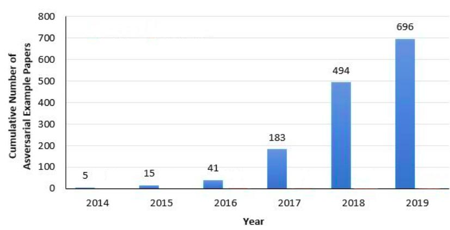
\includegraphics{Figures/figura_01.PNG}
\decoRule
\caption[Estudios publicados]{Estudios publicados asociados a seguridad en redes neuronales \parencite{r62}.}
\label{fig:estudios}
\end{figure}

El documento se compone de la siguiente forma, el capítulo \ref{Definiciones} presenta las definiciones necesarias para comprender el contenido del estudio, en él se explica de manera resumida el funcionamiento de las redes neuronales artificiales y sus tipos más comunes. El capítulo \ref{Ataques} presenta el estado del arte en cuanto a las técnicas de ataques a redes neuronales artificiales, luego el capítulo \ref{Defensa} expone las técnicas de defensas más conocidas. En el capítulo \ref{Experimentos} el lector podrá encontrar los experimentos realizados en el estudio en donde se realizan ataques a sistemas de visión artificial a través de la creación de ejemplos adversarios, utilizando distintas técnicas. También en este capítulo se brinda seguridad a un modelo de clasificación para hacerlo robusto frente a los ataques del experimento. Luego, en el capítulo \ref{Conclusiones} se exponen las conclusiones y resultados del estudio. Finalmente, en el capítulo \ref{Futuro} se presentan los lineamientos futuros sugeridos.


%----------------------------------------------------------------------------------------

\section{Objetivos}

Los objetivos de este estudio son los expuestos a continuación:
\begin{itemize}
\item Presentar un estado del arte de la seguridad en redes neuronales artificiales, exponiendo las distintas técnicas de ataque que pueden ser ejecutadas en contra de este tipo de modelo y presentar investigaciones sobre los tipos de defensas conocidos para hacer frente a dichos ataques.
\item Ejecutar pruebas de ataques en modelos de clasificación propios y presentar resultados que comprueben los estudios analizados.
\item Ejecutar pruebas de ataques en modelos de clasificación importados que sean de uso amplio y conocido para luego presentar resultados que comprueben los estudios analizados.
\item Proponer e implementar una contramedida que permita reducir el impacto de alguno de los tipos de ataques presentados en el estado del arte.
\end{itemize}

%----------------------------------------------------------------------------------------



\chapter{Definiciones} % Main chapter title

\label{Definiciones} % Change X to a consecutive number; for referencing this chapter elsewhere, use \ref{ChapterX}

%----------------------------------------------------------------------------------------
%	SECTION 1
%----------------------------------------------------------------------------------------

\section{Aprendizaje automático}

Las técnicas de aprendizaje automático tienen como objetivo conseguir diferenciar automáticamente patrones usando algoritmos matemáticos. Se pueden distinguir dos tipos de técnicas: supervisadas y no supervisadas. En el aprendizaje supervisado se entrena al ordenador proporcionando ejemplos previamente etiquetados, de forma que el algoritmo usado debe encontrar las fronteras (o acercarse lo más posible) que separan los diferentes tipos de patrones. Las redes neuronales forman parte de este grupo. La figura~\ref{fig:frontera} simboliza la clasificación en un plano en dos dimensiones que se puede obtener con este tipo de algoritmo, donde dependiendo de los valores de entrada se determina a qué clase pertenece (X o +).

\begin{figure}[th]
\centering
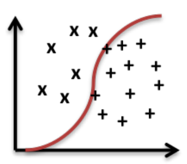
\includegraphics{Figures/figura_02.PNG}
\decoRule
\caption[Frontera de clasificación]{Frontera de clasificación de patrón \parencite{r63}.}
\label{fig:frontera}
\end{figure}


%-----------------------------------
%	SECTION 2
%-----------------------------------
\section{Redes neuronales}

En el campo del aprendizaje automático, las redes neuronales artificiales son una técnica computacional inspirada en la biología, en particular en el funcionamiento de las neuronas, sus conexiones y cómo éstas operan en red para su función. Cada neurona recibe un set de entradas las cuales a través de funciones de activación y parametrizaciones genera una salida, la cual podría convertirse en la entrada de otras neuronas en la red, las que en conjunto son capaces de generar un resultado. Los parámetros que poseen las neuronas se les llama pesos y sesgo (bias), los cuales se asocian a las conexiones de entrada. Estos parámetros son utilizados por su función de activación para generar la salida a partir de los datos de entrada. La figura~\ref{fig:neurona} representa el funcionamiento de una neurona artificial.

\begin{figure}[th]
\centering
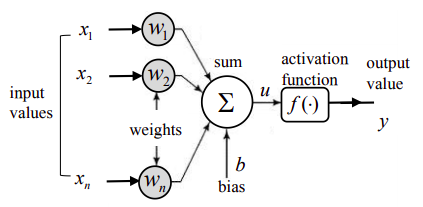
\includegraphics[scale = 1.1]{Figures/figura_03.PNG}
\decoRule
\caption[Neurona]{Neurona artificial \parencite{r64}.}
\label{fig:neurona}
\end{figure}

La salida de la red de neuronas representa posibles resultados de clasificación asociados a un problema. Una red neuronal artificial se compone de capas de neuronas las cuales se conectan entre sí como lo indica la figura~\ref{fig:red}. En la figura las neuronas agrupadas verticalmente representan una capa, cada neurona se conecta con todas las neuronas de la capa anterior y las de la capa siguiente. Cuando se posee al menos una capa oculta, el algoritmo usa arquitecturas computacionales que admiten transformaciones no lineales múltiples e iterativas de datos expresados en forma matricial o tensorial \parencite{r1}

\begin{figure}[th]
\centering
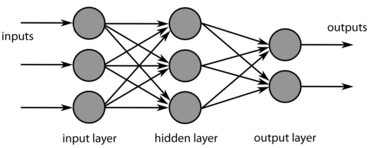
\includegraphics[scale = 1.1]{Figures/figura_04.PNG}
\decoRule
\caption[Neurona]{Red neuronal artificial. Arquitectura simplificada de Perceptrón multicapa \parencite{r13}.}
\label{fig:red}
\end{figure}

Estas redes antes de ser puestas en operación se prepara de la siguiente manera:

\begin{enumerate}
\item Topología de la red: Se busca identificar e implementar topologías óptimas en cuanto a cantidad de capas y neuronas por capas.
\item Parametrización de neuronas: Las redes son entrenadas de manera de conseguir acercarse a la mejor parametrización de pesos por conexión entre neuronas. Para esto se debe contar con una gran cantidad de datos que estén previamente etiquetados, de esta manera se entrena la red ajustando los pesos de cada conexión haciendo tender la red a clasificar correctamente los datos de entrenamiento. A esta técnica en el aprendizaje automático se le llama aprendizaje supervisado, ya que se cuenta con datos de entrada y sus respectivas etiquetas (correcta clasificación) que permite entrenar y validar la eficacia de la red (en cuanto a aciertos).
\item Generalización: Se debe tener precaución respecto a que la red no sobre aprenda. Esto quiere decir que clasifique con un grado alto de exactitud los datos de entrenamiento, pero no así con datos de entrada no pertenecientes a los usados en el entrenamiento.
\end{enumerate}


\section{Redes de aprendizaje profundo}

El aprendizaje profundo es una rama del aprendizaje automático que permite que los modelos computacionales compuestos por múltiples capas de procesamiento con alto nivel de abstracción aprendan de la experiencia y perciban el mundo en términos de jerarquía de conceptos. Utiliza un algoritmo de backpropagation para descubrir detalles intrincados en grandes conjuntos de datos con el fin de calcular la representación de datos en cada capa a partir de la representación en la capa anterior \parencite{r36}. 
Los algoritmos de aprendizaje profundo contrastan con los algoritmos de aprendizaje poco profundo por el número de capas aplicadas a la señal mientras se propaga desde la capa de entrada a la capa de salida. No existe un estándar de facto para el número de capas que convierte a un algoritmo en profundo, pero la mayoría de investigadores en el campo considera que el aprendizaje profundo implica al menos dos capas ocultas \parencite{r2}. Este tipo de algoritmo permite obtener una gran efectividad en la clasificación y ha sido ampliamente utilizad en los últimos años. La figura~\ref{fig:deep} muestra la arquitectura de una red neuronal profunda.

\begin{figure}[th]
\centering
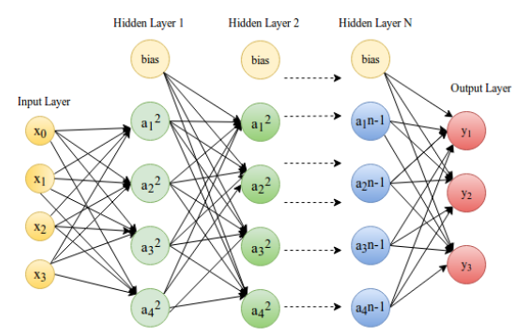
\includegraphics[scale = 1.1]{Figures/figura_05.PNG}
\decoRule
\caption[Neurona]{Red neuronal profunda \parencite{r7}.}
\label{fig:deep}
\end{figure}

Las redes neuronales artificiales no son totalmente confiables, sus salidas no corresponden a algoritmos matemáticos exactos y algunas de sus salidas son erróneas. Estas son entrenadas con grandes volúmenes de datos, de los cuales adquiere conocimiento que utiliza para generalizar sobre nuevas muestras desconocidas para el clasificador. La generalización no resulta eficaz en el total de los casos, pero se considera buena mientras más se acerque al 100\%. En este caso, los fallos se presentan principalmente cuando su entrada es muy distinta a los datos con la que la red fue entrenada.


\section{Visión artificial}

La visión artificial o visión por ordenador es una disciplina científica que incluye métodos para adquirir, procesar, analizar y comprender las imágenes del mundo real con el fin de producir información numérica o simbólica para que puedan ser tratados por un ordenador. Tal y como los humanos usamos nuestros ojos y cerebros para comprender el mundo que nos rodea, la visión artificial trata de producir el mismo efecto para que los ordenadores puedan percibir y comprender una imagen o secuencia de imágenes y actuar según convenga en una determinada situación.
A la hora de aplicar los conceptos teóricos de la visión por ordenador encontraremos siempre interferencias y problemas relacionados con el mundo que nos rodea. Esto es por el mero hecho de que nuestro mundo no es perfecto y los aparatos de medición y captura tampoco lo son. Estos introducen siempre (a mayor o menor cantidad) una distorsión o ruido que contamina la muestra o imagen con la que deseamos trabajar.

\subsection{Redes convolutivas}

Una de las aplicaciones más extendidas de las redes neuronales es la clasificación de imágenes, ya que en la última década ha generado excelentes resultados, llegando a ser muy similar a la clasificación de la vista humana en ciertos contextos. 
Las redes convolutivas son una técnica de las redes neuronales que contiene varias capas ocultas especializadas y con una jerarquía. Las primeras capas pueden detectar líneas curvas y se van especializando hasta llegar a capas más profundas que reconocen formas complejas como un rostro o la silueta de un animal. Este tipo de red neuronal artificial se inspira en el funcionamiento de los campos receptivos de las neuronas en la corteza visual primaria de un cerebro biológico. 

\subsubsection{Entrada de datos}

Las imágenes se transforman en matrices de datos, en donde cada pixel en la foto podría tener 3 dimensiones, según la nomenclatura RGB (Composición del color en términos de la intensidad de los colores) con valores entre 0 y 255. Estos valores a menudo se normalizan para obtener datos entre 0 y 1.  
Por otro lado es recomendable realizar ciertas modificaciones a la imagen de entrada de modo de mejorar la asertividad de la clasificación, generando desde las imágenes de entrada nuevas imágenes producto de rotaciones, acercamientos, traslaciones o de invertir la imagen en algún eje. Esto ayuda a que la red generalice de mejor forma, es decir que pueda clasificar imágenes nuevas distintas a las utilizadas en el entrenamiento.

\subsubsection{Procesamiento}

La figura~\ref{fig:convolutiva} muestra un ejemplo del preprocesamiento de redes convolutivas en donde se extraen las características principales de la imagen para luego ser procesada por una red neuronal como las presentadas previamente (clasificación).

\begin{figure}[th]
\centering
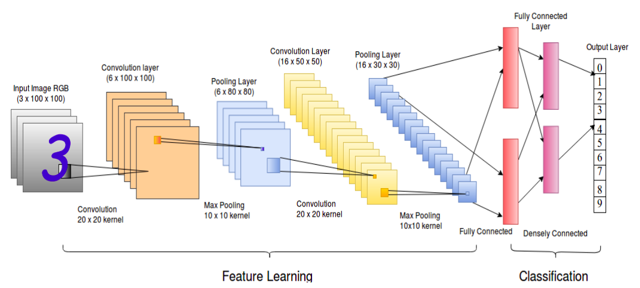
\includegraphics[scale = 0.9]{Figures/figura_06.PNG}
\decoRule
\caption[convolutiva]{Red neuronal convolutiva (CNN) \parencite{r7}.}
\label{fig:convolutiva}
\end{figure}

\subsubsection{Convolución}

Sobre la imagen de entrada se aplican distintos tipos de filtros llamados kernels. La figura~\ref{fig:kernel} muestra una convolución en donde cada píxel de salida es una combinación lineal de los pixeles de entrada. En la convolución se realizan operaciones de productos y sumas entre la capa de partida y los n filtros (o kernel) que genera un mapa de características. Las características extraídas corresponden a cada posible ubicación del filtro en la imagen original. La ventaja es que el mismo filtro sirve para extraer la misma característica en cualquier parte de la entrada, con esto se consigue reducir el número de conexiones y el número de parámetros a entrenar en comparación con una red multicapa de conexión total.

\begin{figure}[th]
\centering
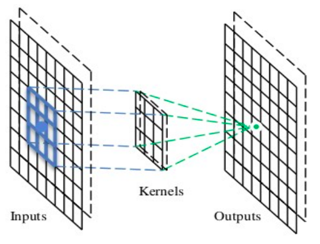
\includegraphics{Figures/figura_07.PNG}
\decoRule
\caption[convolutiva]{Convolución \parencite{r7}.}
\label{fig:kernel}
\end{figure}

\section{Flujo de procesamiento en aprendizaje automático}

Los sistemas de aprendizaje automático poseen un flujo de operación generalizado \parencite{r40} en el cual se puede representar la mayoría de los sistemas en los que se implementa. Este flujo se muestra en la figura~\ref{fig:flujo} en donde un objeto del dominio físico es representado digitalmente a través de cámaras, sensores, eventos de red u otro hardware. Luego la información es procesada en el modelo de aprendizaje automático, el cual entrega una salida, una probabilidad de clasificación u otro tipo de respuesta. El dominio físico recibe esta respuesta y la utiliza para ejecutar alguna acción, como sería el frenar en el caso de un coche de conducción automática frente a una señalética de tránsito. 

\begin{figure}[th]
\centering
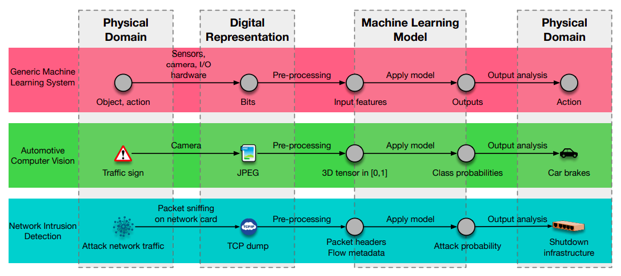
\includegraphics [scale = 0.85]{Figures/figura_08.PNG}
\decoRule
\caption[Flujo genérico] {Flujo genérico de Procesamiento de datos Aprendizaje automático \parencite{r40}.}
\label{fig:flujo}
\end{figure}

\section{Redes generativas con adversario (GAN)}
Las redes generativas con adversario o GAN son redes profundas que compiten en un juego de optimización, en donde existen dos jugadores como se muestran en la figura~\ref{fig:gan2}. Un jugador corresponde a una red neuronal con el rol de “generador”, cuyo objetivo es generar datos sintéticos a partir de una entrada aleatoria, que serán consumidos por el segundo jugador que corresponde a una red neuronal con el rol de discriminador. El discriminador recibe entradas reales (de algún conjunto de datos existente) y sintéticas (generadas por el generador), el discriminador será entrenado en clasificar correctamente las entradas reales y las falsas (sintéticas), mientras el generador será optimizado para crear datos más parecidos a los reales para hacer fallar al discriminador. El procedimiento finaliza cuando el discriminador no logra identificar las entradas sintéticas \parencite{r42}. La figura~\ref{fig:gan1} muestra imágenes creadas por el generador, con excepción de la columna enmarcada en amarillo que corresponde a imágenes reales del conjunto de datos, más similar a las sintéticas, presentada para demostrar que el modelo no memorizó las imágenes, sino que creó nuevas. Una de las aplicaciones de este modelo es la creación de imágenes para aumentar los datos de los entrenamientos y así mejorar la exactitud de algún modelo clasificador.

\begin{figure}[th]
\centering
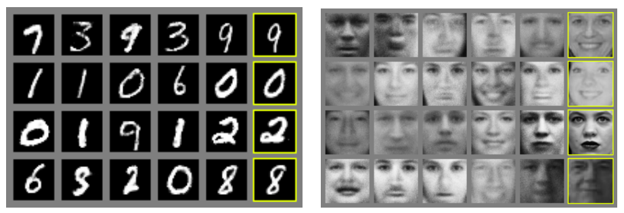
\includegraphics [scale = 0.85]{Figures/figura_09.PNG}
\decoRule
\caption[GAN] {Imágenes creadas por un modelo generador GAN (sintéticas). En amarillo imágenes reales del conjunto de datos \parencite{r42}.}
\label{fig:gan1}
\end{figure}

\begin{figure}[th]
\centering
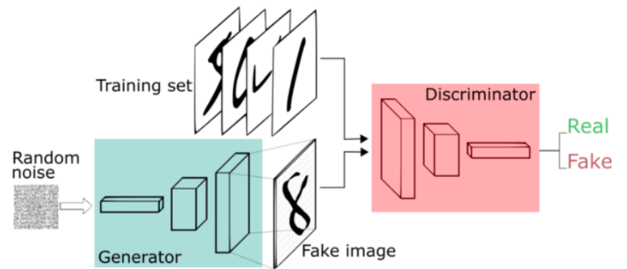
\includegraphics [scale = 0.85]{Figures/figura_10.PNG}
\decoRule
\caption[GAN] {Operación redes generativas con adversario \parencite{r41}.}
\label{fig:gan2}
\end{figure}

Existen variaciones al modelo GAN, como CycleGAN \parencite{r48} con la cual es posible realizar una traducción de imagen a imagen, mapeando en una imagen las características de otra. La figura~\ref{fig:gan3} muestra los resultados obtenidos en un estudio \parencite{r48} en donde una red generadora crea una imagen sintética de estilo fotográfico a partir de una pintura de óleo de Monet (parte superior izquierda), como también transformar imágenes de caballos en cebras o paisajes invernales a veraniegas. 


\begin{figure}[th]
\centering
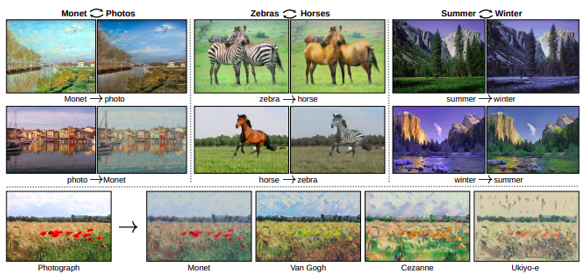
\includegraphics [scale = 0.85]{Figures/figura_11.PNG}
\decoRule
\caption[CycleGAN] {CycleGAN para la traducción de una imagen a otra \parencite{r48}.}
\label{fig:gan3}
\end{figure}

El modelo posee dos funciones de mapeo (una para cada clase de imágenes, ejemplo: caballos y cebras) y también sus respectivos discriminadores Dy y Dx. Dy evalúa si las traducciones de G(X) son indistinguibles a las imágenes del dominio Y, y viceversa Dx con F(Y). Esto en un ciclo el cual comienza con G(X) luego la imagen traducida es vuelta a su estilo original con F(Y) y se ajustan las redes de acuerdo a la pérdida entre la imagen original y la revertida como se indica en la figura~\ref{fig:gan4}.

\begin{figure}[th]
\centering
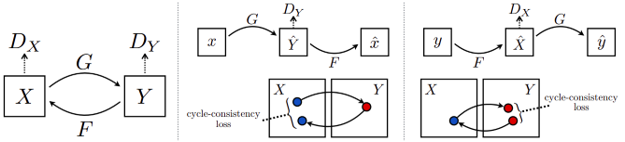
\includegraphics [scale = 0.85]{Figures/figura_12.PNG}
\decoRule
\caption[CycleGAN] {Procedimientos del método CycleGAN \parencite{r48}.}
\label{fig:gan4}
\end{figure}

La figura~\ref{fig:gan5} muestra el ciclo de traducción de imágenes, la primera columna son las imágenes originales, la segunda es la traducida y la tercera es la reconstituida a partir de la traducida. Una de las aplicaciones de este modelo es en el campo de los GIS (sistemas de información geográfica) en el cual como se observa en la última fila de la figura~\ref{fig:gan5}, es posible crear imágenes del estilo de la aplicación de google maps desde fotografías satelitales.

\begin{figure}[th]
\centering
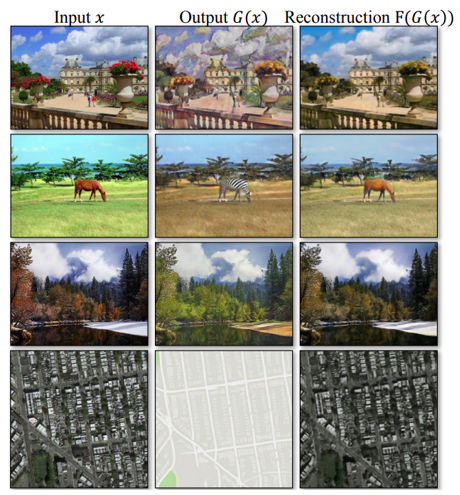
\includegraphics [scale = 0.85]{Figures/figura_13.PNG}
\decoRule
\caption[CycleGAN] {CycleGAN. Traducción de imágenes y reconstrucción de originales \parencite{r48}.}
\label{fig:gan5}
\end{figure} 


\chapter{Ataques a redes neuronales} % Main chapter title

\label{Ataques} % Change X to a consecutive number; for referencing this chapter elsewhere, use \ref{ChapterX}

%----------------------------------------------------------------------------------------
%	SECTION 1
%----------------------------------------------------------------------------------------
La seguridad de los sistemas de aprendizaje automático es vulnerable y sus ataques son conocidos en la literatura como ataques adversarios [adversarial attack] en el cual intencionalmente el atacante intenta alterar la respuesta de un clasificador, ya sea interviniendo el proceso de entrenamiento o bien el proceso de validación u operación. Por ejemplo, puede producir una pequeña perturbación en los datos de entrada \parencite{r49} que llevaría al clasificador entregar un resultado erróneo aun cuando esta perturbación puede resultar imperceptible al ojo humano \parencite{r4}, pero suficiente para que el clasificador arroje una salida errónea o una deseada por el atacante. Lo anterior se puede evidenciar en:
\begin{itemize}

\item En el caso de la visión artificial, en donde existen estudios en los que se simula un ataque a un clasificador de señaléticas de tránsito de vehículos con conducción automática \parencite{r8} para que sean interpretadas de manera errónea por sus sistemas, siendo esta modificación imperceptible para un conductor humano. También se ha llegado a crear ataques físicos, en los cuales la perturbación se lleva a cabo en el mundo físico, en el cual los ataques adversarios también toman efecto \parencite{r12}. 

\item En el caso de los intérpretes de voz como Amazon Alexa o Google Home, donde se han hecho estudios en los cuales dichos sistemas son atacados mediante ultrasonido o ruidos de fondo ocultos \parencite{r17}, e incluso en mensajes que parecen auténticos o canciones \parencite{r31} que poseen comandos de voz ocultos no perceptible por personas.
    
\end{itemize}
En los años recientes varios estudios han demostrado distintas técnicas que provocan fallos en el proceso de clasificación de una red neuronal artificial. Esto ha impuesto el concepto de robustez, el cual señala que tan segura es una red frente a los tipos de ataque que puede recibir. Los ataques adversarios se clasifican en dos grupos, el primero es el llamado “ataque de caja blanca” \parencite{r19} en donde el atacante tiene completo conocimiento sobre el modelo de la red, incluido la topología, entradas, salidas y pesos de sus conexiones. En el segundo llamado “ataque de caja negra” se asume que el atacante sólo tiene acceso a la entrada y salida del modelo, y no sabe nada sobre su topología, pesos de sus conexiones. 
A continuación, se presentan los principales tipos de ataques:




\section{Ataque de extracción de modelo}

El objetivo principal del ataque de extracción de modelo (Model extraction attack) es robar la propiedad intelectual del modelo sin conocimiento previo de los datos y algoritmos de entrenamiento. También podría ser utilizado para ejecutar un ataque de caja negra, siendo usado como modelo sustituto, explotando la capacidad de los ejemplos adversarios de ser transferibles, es decir que un ataque preparado y probado en el modelo sustituto para hacer fallar el clasificador, podría provocar una clasificación errónea en el modelo original \parencite{r9} como lo veremos en adelante. La extracción del modelo el atacante la ejecuta haciendo consultas al clasificador víctima, es decir, a partir de un conjunto de entradas X las cuales son entregada al modelo para obtener las correspondientes predicciones resultados Y. Con estos resultados el atacante podría inferir los valores de los pesos del clasificador \parencite{r33}. La figura~\ref{fig:14} muestra cómo se ejecuta este tipo de ataque a partir de consultas a un clasificador víctima para construir un modelo similar.


\begin{figure}[th]
\centering
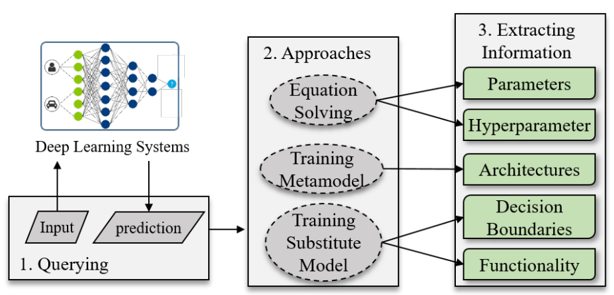
\includegraphics[scale = 0.9]{Figures/figura_14.PNG}
\decoRule
\caption[ ataque de extracción]{Ejecución de un ataque de extracción de modelo \parencite{r32}.}
\label{fig:14}
\end{figure}




\section{Envenenamiento de datos [Poison attack]}

Las redes neuronales artificiales realizan la detección de patrones en base a los datos que se utilizaron en su entrenamiento. En este contexto existe un tipo de ataque llamado envenenamiento de datos o causativos \parencite{r43}, el cual puede ser ejecutado de dos formas que se detallan a continuación, ambas con la intención de provocar que el modelo no pueda clasificar correctamente los datos, ya que se intervino el proceso de aprendizaje \parencite{r34}. 

\begin{itemize}
\item Alteración de las etiquetas del conjunto de datos: En este caso el atacante tiene acceso a los datos con los que se entrenará el clasificador, y procede a modificar las etiquetas, con algún algoritmo o de manera aleatoria.
\item Modificación del contenido de los datos: El atacante podría alterar los datos del conjunto de datos a ser utilizado en el proceso de entrenamiento, incluso de manera imperceptible a una revisión humana. 
\end{itemize}

El ataque podría no querer afectar la eficacia del clasificador excepto para un tipo de patrón determinado en el cual el atacante lograría conducir una respuesta errónea específica (técnica conocida como creación de puerta trasera). Cuando se utiliza un banco de datos públicos para entrenamiento de redes, estamos confiando que aquellos datos y sus etiquetas son correctas. Por otro lado, es muy difícil percibir si los datos fueron manipulados, ya que generalmente se utiliza cientos de miles de datos y etiquetas. La figura~\ref{fig:15} el flujo de operación de un envenenamiento de datos en un modelo de clasificación de imágenes.

\begin{figure}[th]
\centering
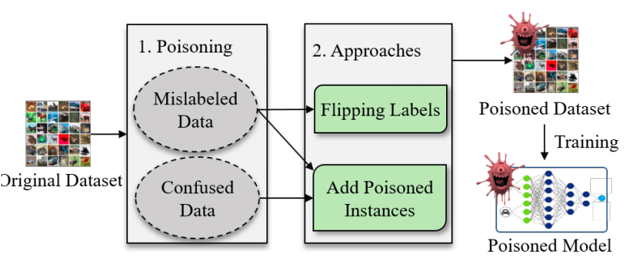
\includegraphics [scale = 0.85] {Figures/figura_15.PNG}
\decoRule
\caption[Envenenamiento de datos]{Envenenamiento de datos, flujo de operación \parencite{r32}
.}
\label{fig:15}
\end{figure}



\section{Ataques adversarios [Adversarial attack]}

Se han realizado estudios respecto a las diferencias entre el razonamiento humano versus el de las redes neuronales para clasificar imágenes, en donde se crean imágenes que no tienen ningún sentido para una persona, pero un clasificador lo identifica con un porcentaje de confidencialidad de hasta un 99,9\% \parencite{r10}. La figura~\ref{fig:16} muestra las imágenes creadas usando algoritmo evolutivo, en donde un clasificador interpreta como un número, cuando en realidad solo hay ruido. En el experimento el autor crea poblaciones iniciales (imágenes) aleatorias equivalentes a ruido, y se itera haciendo mezclas entre los individuos que obtienen mayor confidencialidad en las respuestas del clasificador, llegando a obtener imágenes que no tiene ninguna interpretación a vista de un humano, pero si para la máquina, demostrando que existen diferencias en la forma en que las redes neuronales y los humanos interpretan las imágenes, lo que explica las vulnerabilidades señaladas en adelante.

\begin{figure}[th]
\centering
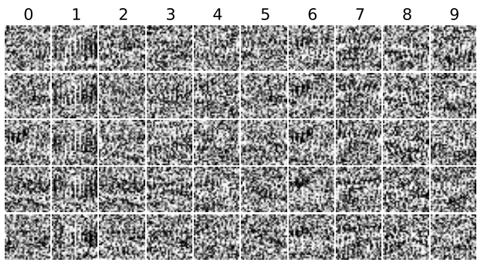
\includegraphics [scale = 0.95] {Figures/figura_16.PNG}
\decoRule
\caption[Ruido interpretado]{Ruido interpretado como números (etiqueta por columna) \parencite{r10}.}
\label{fig:16}
\end{figure}

Los ataques adversarios, también conocidos como exploratorios, son un conjunto de técnicas en la cual el atacante intenta alterar el resultado de un clasificador de un sistema de aprendizaje automático al producir una pequeña perturbación en la entrada \parencite{r4}, cuyo objetivo es que dicha entrada pueda ser clasificada correctamente por un humano, pero no así por un clasificador de inteligencia artificial. Esta perturbación puede resultar ser imperceptible al ojo humano, pero suficiente para que el clasificador arroje una salida errónea o incluso una deseada por el atacante. 

\subsection{Ataque de caja blanca}

En un ataque de caja blanca el atacante tiene acceso al modelo, por lo que además conoce la parametrización de la red como también la arquitectura. Papernote dispuso un marco de trabajo \parencite{r40} el cual permite crear ejemplos adversarios (datos manipulados para el ataque) desde el mismo modelo objetivo del ataque. Por ejemplo, un atacante podría pretender que el clasificador interprete una imagen con el número uno como un cuatro. Para ello analiza la dirección en que debe modificar la imagen resolviendo cuales píxeles de la imagen deben ser modificados. Luego selecciona el tamaño de la perturbación, generalmente buscando el mínimo necesario para lograr el objetivo. Con lo anterior ya se ha creado una nueva imagen que parece ser un número uno, pero este podría ser clasificado como cuatro por el modelo. Si el clasificador no da la respuesta deseada por el atacante, se itera en el ciclo hasta conseguirlo (por ejemplo, aumentando el tamaño de la perturbación). 
Durante el entrenamiento de una red neuronal artificial se suele utilizar la técnica de backpropagation para realizar constantes ajustes a los pesos de las conexiones de la red para obtener los resultados que minimicen la función de pérdida (errores de las clasificaciones). Estos ajustes se propagan desde la capa de salida a las capas anteriores. El gradiente descendente en este proceso de ajuste indica en qué dirección y en qué medida se debe realizar el ajuste para mejorar la clasificación. Esta técnica de aprendizaje es utilizada en forma inversa por el atacante para maximizar el error de la red frente a una entrada modificada maliciosamente, cómo se indicará a continuación. 

Las técnicas más reconocidas para la generación de ataques adversarios son las siguientes \parencite{r19}:

\subsubsection{L-BFGS}

Szegedy \parencite{r4} fue el primero en introducir el término ejemplos adversarios [adversarial example], presentando el siguiente problema de minimización para su generación:

\begin{figure}[th]
\centering
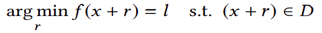
\includegraphics [scale = 0.75]{Figures/formula1.PNG}
\label{fig:f1}
\end{figure}

En la fórmula anterior “x” es el dato original de entrada a la red, “f” es la función de clasificación que representa la operación de la red la cual entrega los resultados del modelo en base a los parámetros de entrada. El ejemplo adversario está representado por “x + r”, que pertenecen al dominio “D” de la red, “l” es la etiqueta incorrecta. El autor plantea el uso del método de optimización L-BFGS para obtener el mínimo valor de “r” capaz de hacer fallar la clasificación, para lo cual hace uso de la gradiente descendiente de la función. Una desventaja de esta técnica es la gran cantidad de cómputo necesaria para obtener el mínimo.



\subsubsection{Fast gradient sign attack}

La técnica de ataque conocida como FGSM (siglas de su nombre en inglés fast gradient sign attack) \parencite{r3} es del tipo “caja blanca” aunque también suele ser efectiva en ataques de caja negra. Genera perturbaciones en la imagen de entrada de la red neuronal artificial utilizando el gradiente descendente, el mismo utilizado en el entrenamiento de la red, pero esta vez en dirección opuesta de manera de generar un nuevo dato de entrada el cual al ser clasificado por el modelo haría fallar su resultado. En el caso de clasificación de imágenes las entradas son matrices de píxeles. Al aplicar la técnica FGSM a partir de una imagen se genera una nueva, cuyos píxeles son modificados para que contribuyan a aumentar el resultado de la función de pérdida de la red, es decir en dirección opuesta a la utilizada en el back propagation para la corrección de pesos, llevando al clasificador a entregar un resultado distinto al que hubiese entregado con la imagen original, pero visualmente imperceptible a una revisión humana.
La generación de la imagen adversaria utilizando FGSM se realiza utilizando el modelo de la red a ser atacada, con la siguiente formula \parencite{r3} utilizando la función de gradiente descendiente:

\begin{figure}[th]
\centering

\includegraphics [scale = 0.75]{Figures/formula2.PNG}
\label{fig:f2}
\end{figure}

\begin{itemize}
    \item $\varepsilon$: Es el factor asociado al grado de la transformación. Indica el tamaño de la perturbación. Toma valores entre 0 y 1.
    \item X: Imagen original (entrada de la red neuronal artificial).
    \item Y: Etiqueta de clasificación correcta para la entrada X.
    \item J($\theta$, X, Y): Función de pérdida utilizada en el entrenamiento. Donde θ representa los parámetros del modelo. 
    \item $\bigtriangledown_x$ J($\theta$, X, Y): Gradiente descendente del clasificador.
\end{itemize}

El objetivo de FGSM es provocar que una entrada haga cruzar la frontera de decisión del clasificador hacia una respuesta incorrecta. La figura~\ref{fig:17} representa esta situación en un modelo de dos clases, en el cual una entrada correspondiente a la clasificación “círculo azul” es modificada de tal forma que el clasificador lo interpreta como “triángulo rojo”.

\begin{figure}[th]
\centering
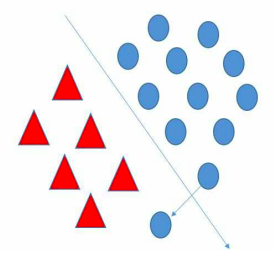
\includegraphics [scale = 0.95] {Figures/figura_17.PNG}
\decoRule
\caption[frontera de decisión]{Traspaso de frontera de decisión. Ataque FGSM \parencite{r4}.}
\label{fig:17}
\end{figure}

En la figura~\ref{fig:18} vemos un ejemplo real de cómo opera el ataque FGSM \parencite{r3}. En él vemos una entrada X que corresponde a un panda, la cual está clasificada correctamente por la red, con una exactitud del 57.7\%. Luego de utilizar el gradiente descendiente del modelo para generar una perturbación de tamaño  la cual es sumada a la imagen inicial, generando una nueva imagen que a vista humana sigue siendo un panda, pero el modelo lo clasifica como otro animal y con una exactitud del 99.3\% la cual es incluso mayor a la de la imagen original. La imagen generada es llamada ejemplo adversario [adversarial example].

\begin{figure}[th]
\centering
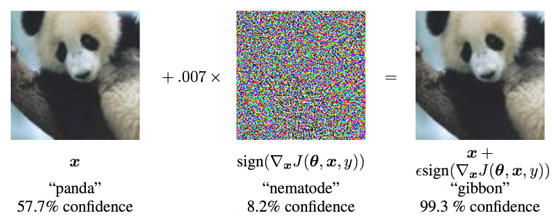
\includegraphics [scale = 0.95] {Figures/figura_18.PNG}
\decoRule
\caption[FGSM]{Ejemplo de ataque FGSM \parencite{r3}.}
\label{fig:18}
\end{figure}

La figura~\ref{fig:19} muestra un ataque a una red neuronal artificial de clasificación de imágenes de dígitos numéricos. En ella se muestra para un conjunto de datos de entrada, distintos valores de $\varepsilon$, para presentar como se ve afectada la imagen y la clasificación a medida que aumenta el tamaño de la perturbación. Un $\varepsilon$ igual a cero representa la imagen original, la cual fue correctamente clasificada. Desde $\varepsilon$ 0,05 el algoritmo clasifica mal, pero la imagen no parece haber sido manipulada. A medida que aumenta $\varepsilon$ la imagen muestra colores sospechosos para la vista humana, no así para el modelo, ya que incrementa la probabilidad de que este arroje una respuesta errónea.

\begin{figure}[th]
\centering
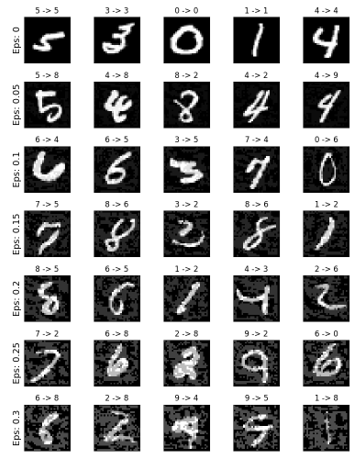
\includegraphics [scale = 1] {Figures/figura_19.PNG}
\decoRule
\caption[MNIST]{Distintos valores eps sobre MNIST \parencite{r3}.}
\label{fig:19}
\end{figure}



\subsubsection{Método de clase objetivo [Target class method]}

Este ataque puede también ser dirigido no solo para hacer fallar la clasificación, sino también para que esta clasifique en un valor deseado por el atacante. El método de clase objetivo es una variante de FGSM \parencite{r37} en el cual el atacante define la respuesta errónea que desea recibir del clasificador y busca las perturbaciones necesarias para dicho objetivo. La figura~\ref{fig:20} muestra un ejemplo de esto, en donde con una imagen del dígito 1 el atacante itera en la confección del ejemplo adversario hasta conseguir que el modelo lo clasifique con el valor 4.

\begin{figure}[th]
\centering
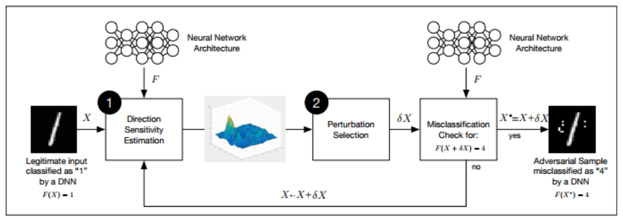
\includegraphics [scale = 0.9] {Figures/figura_20.PNG}
\decoRule
\caption[adversario dirigido]{Ejemplo adversario dirigido \parencite{r24}.}
\label{fig:20}
\end{figure}

\subsubsection{Método de clase objetivo [Método Jacobiano]}

Este método permite generar ataques dirigidos, es decir cuando el atacante desea que la red arroje un resultado específico de su interés. Papernote \parencite{r13} plantea en su investigación el uso del método Jacobiano como una forma de obtener la dirección de sensibilidad, es decir el Jacobiano de la función de aprendizaje (matriz de derivadas parciales). La construcción del ejemplo adversario en este método se realizan utilizando la matriz Jacobiana para crear el mapa de perturbaciones necesarias para obtener la salida deseada de la red. Para dirigir la salida de la red se itera observando cómo las perturbaciones en la entrada afectan la salida. El mapa de prominencias (map saliency) indica en qué píxeles de la entrada (en el caso de clasificación de imágenes) la red presenta más sensibilidad para inclinar su resultado a una clase determinada. La figura~\ref{fig:21} muestra un mapa de prominencias asociada a una imagen de 28x28 píxeles, el valor absoluto del eje Y indica que perturbaciones en la entrada obtendría mayor efectividad de llevar a la salida a un resultado deseado.

\begin{figure}[th]
\centering
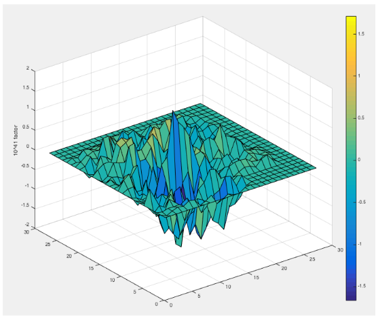
\includegraphics [scale = 1] {Figures/figura_21.PNG}
\decoRule
\caption[Mapa]{Mapa de protuberancias que indica en cuales píxeles de una imagen de 28x28 existe mayor sensibilidad en el clasificador \parencite{r13}.}
\label{fig:21}
\end{figure}

La figura~\ref{fig:22} indica resultados de estudio citado \parencite{r13}, en donde con el método Jacobiano se dirige el ataque para obtener un resultado específico en cada dígito, cuya imagen original se encuentra en la diagonal. El conjunto de datos utilizado es el MNIST de detección de dígitos. El ataque logró para cada dígito de entrada dirigirlo a cada una de las clases del clasificador. Se observa que para algunos dígitos se requiere mayor manipulación que para otros, como por ejemplo lograr que un 5 sea clasificado como un 1. Por otro lado, hay casos como el llevar al clasificar a confundir un 3 con un ocho, en donde prácticamente la perturbación es imperceptible a la vista humana. El dígito 1 resultó ser en promedio el más vulnerable de llegar a ser clasificado como cualquier otro dígito, con menores alteraciones.

\begin{figure}[th]
\centering
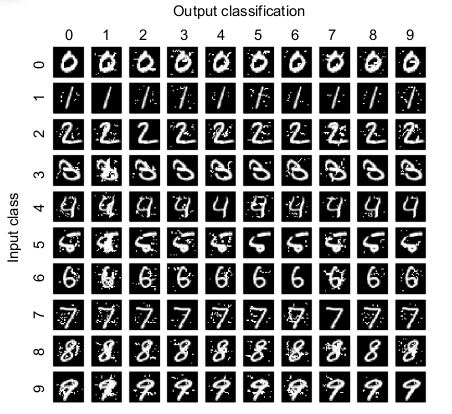
\includegraphics [scale = 1] {Figures/figura_22.PNG}
\decoRule
\caption[Mapa]{Perturbaciones dirigidas con metodo Jacobiano \parencite{r13}.}
\label{fig:22}
\end{figure}




\subsubsection{Método de clase objetivo [Ataque CW]}
Carlini y Wagner \parencite{r55} propusieron una técnica de ataque que no utiliza el gradiente descendiente de un modelo entrenado, en su lugar utiliza parámetros asociados a una regresión del clasificador. Ellos experimentaron con diferentes formulaciones de la función objetivo de la optimización para encontrar ejemplos adversarios en ataques de caja blanca. Descubrieron que minimizar una suma ponderada de la norma de perturbación y una función de pérdida de clasificación particular, Losscw, ayuda a lograr ataques más imperceptibles. Definieron la función Losscw no directamente sobre las probabilidades emitidas por clasificador, sino sobre los logits. Este se define como el logaritmo neperiano (log) del cociente de probabilidades de dos sucesos. En términos generales, Losscw se define de la siguiente manera: 

\begin{figure}[th]
\centering
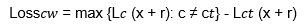
\includegraphics [scale = 0.75]{Figures/formula3.PNG}
\label{fig:f3}
\end{figure}

Donde Lc (·) es el logit para la clase c. Maximizar la función de pérdida ($Loss_{c_w}$) aumenta la probabilidad de la clase objetivo, ct, y disminuye la probabilidad de otras.




\subsubsection{AGN redes generativas adversarias}

Un estudio reciente \parencite{r56} propone entrenar una GAN (redes neuronales generativas) que toma una imagen como entrada y genera una versión perturbada de la misma imagen que estaría mal clasificada para crear imágenes perturbadas por el adversario que conducen a una clasificación errónea. Estos ataques solo requieren que las perturbaciones tengan una pequeña norma y permitan que las perturbaciones cubran solo una pequeña porción específica de la imagen y múltiples objetivos (por ejemplo, generar anteojos que conduzcan a una clasificación errónea y parezcan realistas). 
Las GAN proporcionan un marco de trabajo para entrenar una red neuronal, denominada generador (G), para generar datos que pertenecen a una distribución (cercana a la real). G mapea muestras de una distribución Z de vectores d-dimensionales de reales entre -1 y 1 a muestras de la distribución objetivo. Para entrenar a G, se usa otra red neuronal, llamada discriminador (D). El objetivo de D es discriminar entre muestras reales y generadas. Por lo tanto, el entrenamiento puede conceptualizarse como un juego con dos jugadores, D y G, en el que D está entrenado para emitir 1 en ejemplos reales y 0 en muestras generadas, y G está entrenado para generar salidas que son (mal) clasificadas como reales por D. En la práctica, el entrenamiento se desarrolla de forma iterativa y alterna entre la actualización de los parámetros de G y D mediante backpropagation.

\subsection{Ataques de caja negra}

A diferencia del ataque del tipo caja blanca, en donde el atacante tiene acceso al modelo, lo que le facilita su objetivo, en los ataques de caja negra el atacante sólo tiene acceso a introducir una entrada a la red y a obtener la clasificación realizada por el modelo. A pesar de esta dificultad, estudios \parencite{r4} han demostrado que las redes neuronales artificiales son vulnerables a los ejemplos adversarios generados en modelos distintos, pero con mismas clases de salida. Esto quiere decir que el atacante puede crear un modelo propio de clasificación llamado “modelo sustituto”, y con este crear los ejemplos adversarios que usará para hacer fallar la clasificación de la red neuronal a ser atacada. La creación de los ejemplos adversarios se realizan con el gradiente descendiente tal como las técnicas de caja blanca. Esta propiedad de los modelos se le llama “transferibilidad”. Estos ataques suelen ser algo menos efectivos que en los de caja blanca, ya que en el caso de los ataques de caja negra existe una probabilidad alta en la que el ejemplo adversario no surja el efecto deseado por el atacante, dependiendo del modelo de origen, modelo destino, datos de entrenamiento. Cuando la red neuronal maliciosa es entrenada con los mismos datos con la que fue entrenada la red inicial la probabilidad que esta obtenga fronteras de clasificación similar a la red neuronal original es más alta, haciendo más efectivo el ataque. Sin embargo, si no se cuenta con estos datos, se puede usar el modelo original como caja negra para etiquetar imágenes de ejemplo o sintéticas y con estos datos entrenar el modelo sustituto. El atacante buscando mejorar su resultado podría crear varios modelos sustitutos distintos donde probar sus ejemplos adversarios, de modo de identificar cuáles de estos generalizan mejor las fallas, seleccionando así el ejemplo adversario más efectivo para lograr su cometido. Las técnicas de ataque de caja negra son más costosas en comparación a las de caja blanca, debido a que el atacante debe crear uno o varios modelos sustitutos para generar un ejemplo adversario. 
Estudios han demostrado que esta transferibilidad de los ejemplos adversarios creados desde un modelo sustituto también son efectivo en otros tipos de técnicas de aprendizaje automático como regresión logística, máquinas de vectores de soporte (SVM), árboles de decisión y K vecinos más cercanos (KNN) \parencite{r9}.




\subsection{Ataques en el mundo real}

Los ataques adversarios no solo son ejecutables de manera digital, estudios \parencite{r51, r52, r54, r56} han demostrado que es posible que surtan efecto en el mundo físico, aunque los métodos estándar para generar ejemplos de adversarios para redes neuronales no engañan constantemente a los clasificadores de redes neuronales en el mundo físico debido a una combinación de cambios como los puntos de vista, ruido de cámara y otras transformaciones naturales, lo que impone un desafío adicional que dificulta su aplicación en sistemas del mundo real \parencite{r52}.

\subsubsection{Imágenes impresas}

Una Investigación realizada en el 2018 realizó pruebas con imágenes ejemplos adversarios impresas. Se utilizó una cámara de un teléfono móvil, cuyas imágenes capturadas alimentaban la entrada de un modelo de red de aprendizaje profundo. Se utilizó impresiones (fotografías) de imágenes originales, como también de ejemplos adversarios, y se pudo observar como el clasificador en una gran fracción de los casos fue vulnerado. También se demostró que los ataques de tipo caja negra son efectivos en este contexto. La figura~\ref{fig:23} muestra uno de los experimentos en donde se tomó una imagen del conjunto de datos, la cual una vez impresa la original es correctamente clasificada por el modelo a través de la cámara del teléfono móvil (fotografía izquierda). Luego se imprimen los ejemplos adversarios, y son clasificados erróneamente por el modelo.

\begin{figure}[th]
\centering
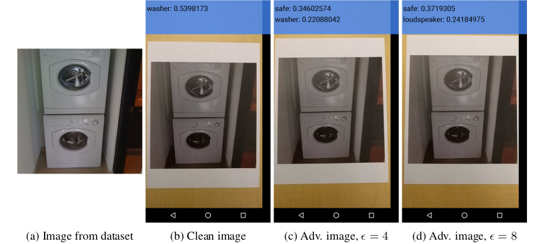
\includegraphics [scale = 1] {Figures/figura_23.PNG}
\decoRule
\caption[Mundo físico]{Ejemplos adversarios en el mundo físico. imágenes impresas \parencite{r51}.}
\label{fig:23}
\end{figure}

\subsubsection{Objetos 3D}

Estudios han realizado ataques generando ejemplos adversarios en formato 3D usando impresoras de dicha tecnología \parencite{r52} logrando hacer fallar la clasificación de un modelo de aprendizaje profundo. La figura~\ref{fig:24} muestra los objetos creados, son esculturas de tortugas, las cuales un hacen fallar la clasificación en un modelo de aprendizaje profundo. La primera fila son impresiones 3D originales. El autor implementa un tipo de algoritmo que permite, a partir de las técnicas de ataques antes mencionadas, crear ejemplos adversarios en 3D, técnica que llamó Expectation Over Transformation (EOT).

\begin{figure}[th]
\centering
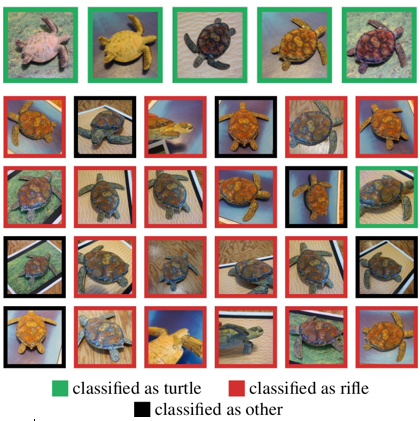
\includegraphics [scale = 1] {Figures/figura_24.PNG}
\decoRule
\caption[Ejemplos adversarios en el mundo físico. Impresión 3D]{Ejemplos adversarios en el mundo físico. Impresión 3D \parencite{r52}.}
\label{fig:24}
\end{figure}

\subsubsection{Señaléticas de tránsito}

Existen investigaciones asociadas a señaléticas de tránsito, en donde una red de aprendizaje profundo de visión artificial de un sistema de conducción automática de coches es sometida a señaléticas que han sido alteradas con parches blancos y negros logrando hacer fallar su clasificación en un 100\% en imágenes y 84.8\% en cuadros capturados por un video en un coche en movimiento,  llevando al sistema a interpretar una señalética pare como una de límite de velocidad 45 \parencite{r54}. Para lograr estas perturbaciones se utiliza una técnica de ataque llamada por el autor como “Perturbaciones físicas robustas” [Robust Physical Perturbations], que permite generar ejemplos adversarios bajo diferentes condiciones físicas. La figura~\ref{fig:25} presenta el resultado de una de las señaléticas creadas (imagen de la derecha) y se compara con una señalética que ha sido pintada con un grafiti, para evidenciar que una modificación como estas suele ser desatendidas por los conductores.

\begin{figure}[th]
\centering
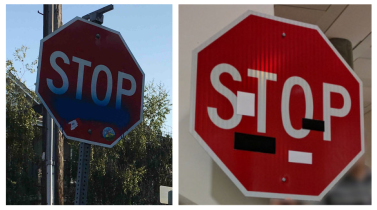
\includegraphics [scale = 1] {Figures/figura_25.PNG}
\decoRule
\caption[Ejemplos adversarios en el mundo físico. Señalética de vehículos]{Ejemplos adversarios en el mundo físico. Señalética de vehículos \parencite{r54}.}
\label{fig:25}
\end{figure}

\subsubsection{Evasión de detección facial}

Estudios realizados el año 2019 \parencite{r56} han logrado crear gafas imprimibles con un diseño y colores tal que permiten a un individuo evadir los sistemas de detección facial. Este accesorio fue diseñado utilizando un método similar a las redes generativas con adversario (GAN) con el que se entrenó una red generadora la cual crea ejemplos adversarios dirigidos, es decir que el clasificador entrega un resultado erróneo deseado por el atacante. Se toma como entrada un conjunto de imágenes de gafas. La figura~\ref{fig:26} muestra a la izquierda las gafas resultantes, que permitirían a una persona evadir la detección facial. A la derecha las imágenes originales del conjunto de datos.

\begin{figure}[th]
\centering

\includegraphics [scale = 0.9] {Figures/figura_26.PNG}
\decoRule
\caption[Ejemplos adversarios de gafas]{Ejemplos adversarios en el mundo físico. Izquierda: ejemplos adversarios de gafas. Derecha: gafas originales del conjunto de datos \parencite{r56}.}
\label{fig:26}
\end{figure}

Con la imagen de gafas del tipo ejemplo adversario se prueba la detección facial (conjunto de datos PubFig) como se muestra en la figura~\ref{fig:27}, a la izquierda la imagen original que fue reconocida por la red de aprendizaje profundo (VGG143) con probabilidad 100\%, mientras que la imagen derecha que posee los lentes adversarios (montaje digital) reconoció la persona con probabilidad menor al 0.01\%. 

\begin{figure}[th]
\centering
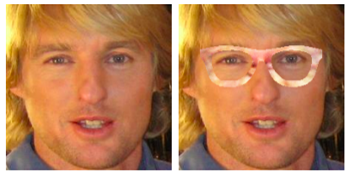
\includegraphics [scale = 1] {Figures/figura_27.PNG}
\decoRule
\caption[Imagen del actor Owen Wilson, montaje gafas de evasión de detección facial]{Ejemplos adversarios en el mundo físico. Imagen del actor Owen Wilson, montaje gafas de evasión de detección facial \parencite{r56}.}
\label{fig:27}
\end{figure}

Para implementar el ataque a nivel físico, los lentes fueron impresos y probados en personas como lo muestra la figura~\ref{fig:28}. En este experimento se logró que la persona situada en la fila superior suplante la identidad de la persona ubicada inmediatamente bajo ella.

\begin{figure}[th]
\centering
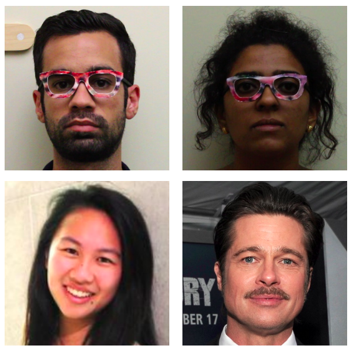
\includegraphics [scale = 1] {Figures/figura_28.PNG}
\decoRule
\caption[Suplantación de identidad]{Ejemplos adversarios en el mundo físico. Suplantación de identidad \parencite{r56}.}
\label{fig:28}
\end{figure}

\subsection{Ataques adversarios en la actualidad}
\subsubsection{Febrero 2020: Mcafee y ataque a señalética de tránsito}
La empresa Mcafee posee un área de investigación llamada Mcafee-labs, la cual recientemente liberó un artículo \parencite{r53} de una investigación asociada a la manipulación de señalética de tránsito para provocar fallos en los sistemas ADAS (Advanced Driver Assist Systems) de conducción automática utilizados por cerca de 40 millones de vehículos, incluidos los coches Tesla, con el fin de poner en discusión la seguridad de los sistemas de inteligencia artificial. Continuaron con los estudios realizados en una investigación de otro grupo de científicos \parencite{r52} que crearon un ejemplo adversario físico de una señalética pare. El equipo luego de 18 meses de trabajo logró crear señaléticas de velocidad máxima que son interpretadas erróneamente por los sistemas ADAS por una velocidad máxima mayor. 
La figura~\ref{fig:29} muestra una las imágenes resultantes. El clasificador de ADAS identifica esta señalética como una de velocidad máxima de 85 en lugar de 35. La figura~\ref{fig:30} es una fotografía del hardware de dicho sistema, el cual se utilizó en los experimentos de Mcafee. 

\begin{figure}[th]
\centering
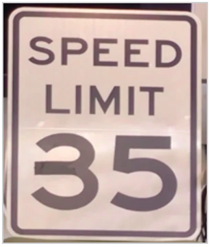
\includegraphics [scale = 1] {Figures/figura_29.PNG}
\decoRule
\caption[Ejemplo adversario de imagen de límite de velocidad]{Ejemplo adversario de imagen de límite de velocidad interpretado como velocidad máxima 85 \parencite{r53}.}
\label{fig:29}
\end{figure}

\begin{figure}[th]
\centering
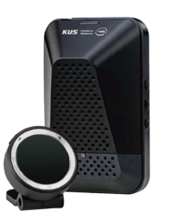
\includegraphics [scale = 1] {Figures/figura_30.PNG}
\decoRule
\caption[Hardware de sistema ADAS (Advanced Driver Assist Systems) ]{Hardware de sistema ADAS (Advanced Driver Assist Systems) \parencite{r53}.}
\label{fig:30}
\end{figure}
Lo expuesto es una señal de precaución para los conductores de vehículos autónomos ya que muchos conductores sobreestiman esta tecnología.




\subsubsection{Junio 2020: Caso Burger King}
Recientes noticias \parencite{r57} relatan una situación vivida por usuarios de vehículos de conducción automática Tesla, los cuales ante una señal vertical con el logo de Burger King provocaba que el vehículo se detuviera, ya que interpretaba la imagen como un signo pare. No hay antecedentes sobre si el anuncio publicitario fue preparado para provocar la detención de los vehículos, pero lo ocurrido demuestra lo distinto que funciona la interpretación de los sistemas de aprendizaje automático y la vista humana. Afortunadamente esta situación no provocó accidentes, pero dejó en evidencia que esta tecnología no está completamente desarrollada. La noticia se viralizó en Norteamérica y ante esto Burger King publicó en sus redes sociales “La inteligencia artificial sabe lo que anhelas”.
Es importante saber que la automatización de estos vehículos se considera en el Nivel 2 de automatización de las capacidades de conducción, lo que significa que es de un tipo asistida por el conductor y no completamente autónoma.

\begin{figure}[th]
\centering
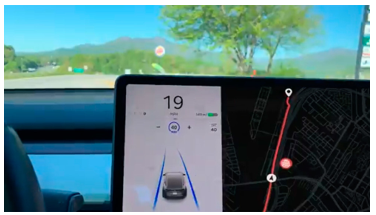
\includegraphics [scale = 1] {Figures/figura_31.PNG}
\decoRule
\caption[Vehículo de conducción automática confunde una publicidad con signo pare]{Vehículo de conducción automática confunde una publicidad con signo pare \parencite{r57}.}
\label{fig:31}
\end{figure}


\chapter{Defensa frente a ataques adversarios} % Main chapter title

\label{Defensa} % Change X to a consecutive number; for referencing this chapter elsewhere, use \ref{ChapterX}

%----------------------------------------------------------------------------------------
%	SECTION 1
%----------------------------------------------------------------------------------------
A la fecha en que se redacta este documento no existe una solución definitiva que permita blindar completamente a una red neuronal de los ataques presentados en el presente documento. Las siguientes son las dificultades que enfrenta la elaboración y diseño de defensas \parencite{r7}:
\begin{itemize}
    \item La elaboración de un ejemplo adversario es un proceso de optimización complejo que no es lineal ni convexo para la mayoría de los modelos de aprendizaje automático. La falta de herramientas teóricas adecuadas para describir la solución a estos complejos problemas de optimización hace que sea aún más difícil hacer cualquier argumento teórico de que una defensa particular es robusta frente a un conjunto de ejemplos adversarios.

    \item Las técnicas de aprendizaje automático están diseñadas para entregar respuesta a cada entrada. Una modificación considerable del modelo para incorporar robustez frente a los ejemplos adversarios puede cambiar el objetivo elemental del modelo.
\end{itemize}
Lo anterior ha provocado un juego cíclico entre el atacante y el defensor del clasificador \parencite{r49}. Por ejemplo, en un sistema de filtro de correos no deseados, el atacante con el fin de hacer fallar la detección añade nuevas palabras al correo. Cuando el defensor se da cuenta que su filtro fue vulnerado, modifica su algoritmo añadiendo las nuevas palabras, pero el atacante vuelve a modificar su correo \parencite{r50}. Una situación similar ocurre en la defensa de otros tipos de sistemas de aprendizaje profundo.
Han surgido ciertas técnicas que minimizan algunos tipos de ataques. Las soluciones se dividen principalmente en tres grupos \parencite{r39}: 
\begin{enumerate}
    \item Modificación de datos de entrenamiento para hacer más robusto al clasificador frente a un ejemplo adversario.
    \item Modificación del proceso de entrenamiento del clasificador para reducir la magnitud de los gradientes y así dificultar la creación de ejemplos adversarios.
    \item Intentar remover el ruido de las entradas para volver menos efectivo un ejemplo adversario. 
\end{enumerate}

\section{Entrenamiento con ejemplos adversarios [Adversarial training]}
Esta técnica de defensa consiste en crear ejemplos adversarios y luego agregarlos al conjunto de datos de entrenamiento con la etiqueta correcta de clasificación \parencite{r19}. De esta forma el clasificador al verse enfrentado al ataque clasificará correctamente la entrada. Esta técnica es considerada como un acercamiento a fuerza bruta, donde el defensor genera un conjunto de ejemplos adversarios, luego dichas imágenes son introducidas a la fase de entrenamiento agregando estas al conjunto de datos original, la técnica suele ser más efectiva al aplicar también aumento del conjunto de entrenamiento, aplicando funciones como rotación, giro horizontal o vertical, zoom, cambios de perspectivas y desplazamiento sobre los datos existentes. Un inconveniente de esta técnica es que tiende a sobre aprender al ataque específico utilizado en el tiempo de entrenamiento, presentando dificultad de generalizar sobre los ejemplos adversarios similares (no utilizados en el entrenamiento). Esto se puede mejorar agregando ruido a las imágenes \parencite{r6}. Los ejemplos adversarios creados para entrenar la red se producen utilizando la o las técnicas de las cuales se desea proteger el modelo. Este método de defensa solo es efectivo en ataques del tipo caja blanca, ya que este es fácilmente vulnerable con entradas generadas en un modelo sustituto (ataque de caja negra) \parencite{r7}. 

\section{Redes generativas con adversario (GAN) como defensas}
Una investigación reciente \parencite{r39} propuso la utilización de redes generativas con adversario (GAN) como defensa en la cual, se prepara al generador a crear muestras que se asemejan a los datos de entrenamiento. Por lo tanto, se espera que las muestras legítimas estén cerca de algún punto en el rango del generador, mientras que las muestras adversas estarán más lejos. Para lograr esto el autor propone proyectar la entrada sobre el rango del generador, como se muestra en la figura~\ref{fig:32}. Además, el autor indica que en algunos casos esta transformación disminuye el ruido de la imagen y vuelve más débiles los ejemplos adversarios.

\begin{figure}[th]
\centering
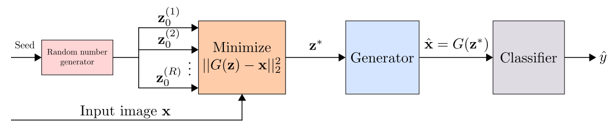
\includegraphics[scale = 0.9]{Figures/figura_32.PNG}
\decoRule
\caption[Redes generativas con adversario (GAN) como defensas]{Redes generativas con adversario (GAN) como defensas \parencite{r39}.}
\label{fig:32}
\end{figure}

Esta defensa pretende ser efectiva tanto a ataques de caja blanca o caja negra. Su desventaja es que baja la efectividad de clasificación del modelo.


\section{Destilación como defensa}

Dentro de las técnicas de protección, existe una categoría en la cual se realiza un enmascaramiento de gradientes. La mayoría de los ataques de caja blanca operan computando gradientes del modelo y, por lo tanto, fallan si es imposible calcular gradientes útiles. El enmascaramiento de gradiente consiste en hacer que el gradiente sea inútil, ya sea cambiando el modelo de alguna manera que lo hace imperceptible o que tenga gradiente cero en la mayoría de los lugares.
La destilación es una técnica de entrenamiento formulada para transferir conocimiento de un modelo de aprendizaje profundo a otro, con el fin de reducir la complejidad computacional transfiriendo el conocimiento de arquitecturas más grandes a arquitecturas más pequeñas \parencite{r61}. Estudios recientes propusieron una variante de dicha técnica como defensa frente a ejemplos adversarios, en donde se utiliza el conocimiento extraído de un modelo para mejorar su propia robustez. en donde se entrena al clasificador en dos rondas. La figura~\ref{fig:33} muestra el proceso de destilación, en donde se entrena una red de como comúnmente se hace, y luego se utiliza su vector de predicción como etiqueta en una segunda red para cada dato de entrenamiento. Esto tiene el efecto de generar una red más fluida y reducir la amplitud de los gradientes alrededor de los puntos de entrada, lo que dificulta que los atacantes generen ejemplos adversarios \parencite{r24}. Si los gradientes son altos, la elaboración de ejemplos adversarios es más fácil porque pequeñas perturbaciones inducen altas variaciones en la clasificación del modelo. 
Si bien la destilación defensiva es eficaz en ataques de caja blanca, no protege adecuadamente contra los ataques de caja negra con ejemplos adversarios transferidos desde otro modelo \parencite{r28}. Por otra parte, este tipo de defensa sólo es eficaz frente a ataques que se formulan a partir del gradiente descendiente, siendo aún vulnerable a otros tipos de ataques, como por ejemplo, los realizados por regresión de los modelos como se expuso en estudios posteriores \parencite{r55}. 

\begin{figure}[th]
\centering
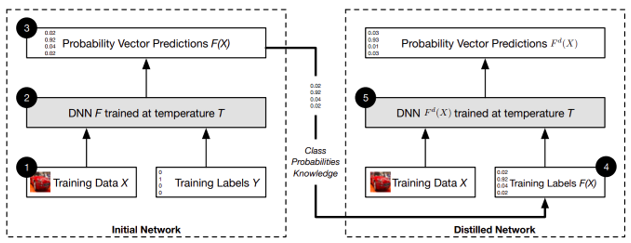
\includegraphics[scale = 0.9]{Figures/figura_33.PNG}
\decoRule
\caption[Entrenamiento con técnica de destilación ) como defensas]{Entrenamiento con técnica de destilación como defensa \parencite{r24}.}
\label{fig:33}
\end{figure}

\section{Agregar la clasificación NULL}

Otra técnica de protección consiste en agregar una nueva salida de la red llamada NULL, en la cual se entrena la red para que pueda clasificar los ejemplos adversarios en esta categoría. La figura~\ref{fig:34} muestra cómo opera este método de defensa con imágenes del conjunto de datos MNIST. La imagen superior (dígito cero) corresponde a la original, mientras que las inferiores son ejemplos adversarios. En la figura se compara un clasificador tradicional versus cómo clasifica el modelo con la salida NULL. cuando la clase NULL toma valores por sobre cierto valor (a determinar en cada modelo) es posible detectar un ataque. Este mecanismo de defensa es efectivo frente a los ataques del tipo caja negra, ya que rompe la transferibilidad de los ejemplos adversarios \parencite{r7} al agregar la nueva clase NULL al modelo. La desventaja de este mecanismo es que baja la efectividad de clasificación del modelo.


\begin{figure}[th]
\centering
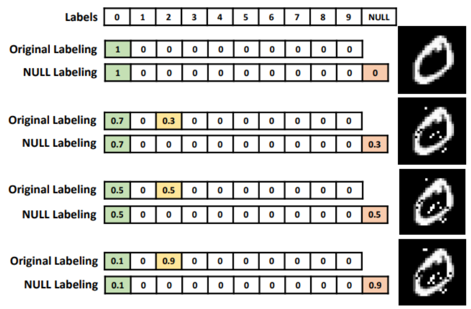
\includegraphics{Figures/figura_34.PNG}
\decoRule
\caption[Clasificación NULL de ejemplos adversarios]{Clasificación NULL de ejemplos adversarios \parencite{r7}.}
\label{fig:34}
\end{figure}

\section{Arquitectura de software resiliente}
Un estudio reciente de la Scuola Superiore Sant’Anna, Pisa \parencite{r5}, proponen un modelo para brindar seguridad a los sistemas de aprendizaje profundo desde la mirada de la arquitectura de software, apuntando principalmente a los sistemas críticos, con objetivos como robustez, tolerancia a fallos y lo más certificable posible, ya que su mal funcionamiento en este tipo de sistema podría poner en riesgo vidas humanas o desatar un desastre medio ambiental. Además, en los sistemas críticos deben reaccionar a los eventos en un tiempo predecible. Una salida de control entregada demasiado tarde podría ser inútil o incluso peligroso (como ejemplo, un comando de frenado en un auto con conducción automática). Esto significa que estos sistemas deben ser verificables no solo en el dominio funcional, sino también en el dominio del tiempo. El estudio propone un sistema de alta disponibilidad de clúster de servidores. Este sistema puede ser activo-pasivo o activo-activo, dependiendo de cómo se requiera administrar los recursos. 
Una de las dificultades que existen en certificar como sistema crítico un sistema de aprendizaje profundo es en cuanto a lo siguiente:
\begin{itemize}
    \item Los resultados obtenidos de una red neuronal artificial no son 100\% confiables. 
    \item Los sistemas basados en redes neuronales artificiales comúnmente son desarrollados usando marcos de trabajos como TensorFlow, Keras o Caffe que facilitan su implementación, permitiendo crear modelos óptimos de redes neuronales con pocas líneas de código. Estos no son compatibles con el estándar de codificación usado en certificaciones de sistemas de software críticos. 
    \item Estos sistemas generalmente se ejecutan en sistemas operativos como Linux, los cuales no son sistemas operativos de tiempo real, comúnmente usados en sistemas críticos.
\end{itemize}
En estos sistemas se hace necesario contar con este dominio no certificable, ya que los controladores de dispositivo (como la GPU) y software necesarios para la operaciones de una red neuronal artificial solo están disponibles para sistemas operativos enriquecidos, y no de tiempo real utilizados y exigido por certificaciones de sistemas críticos. Para poder resolver estas desventajas el estudio propone la arquitectura presentada en la figura~\ref{fig:35}, la cual posee un dominio de software no certificable en los estándares de sistemas críticos, que se compone de 3 modelos de redes neuronales distintos (aunque pudiesen ser más) que clasifican en paralelo las entradas, los cuales se ejecutan en servidores independientes con sistemas operativos enriquecidos (ejemplo Linux). También cuenta con una máquina con sistema operativo de tiempo real (RTOS) que cumple funciones de control, monitoreo y consolidación de los resultados obtenidos por los modelos de redes neuronales artificiales llamado “Dominio crítico” que posee infraestructura y software certificable. Además, incluye una capa que cumple la función de hipervisor de estas máquinas, monitoreando disponibilidad y seguridad. El Hipervisor si detecta un comportamiento no esperado en las máquinas de SO puede ejecutar procedimientos de recuperación. La infraestructura y software del Hypervisor es certificable.

\begin{figure}[th]
\centering
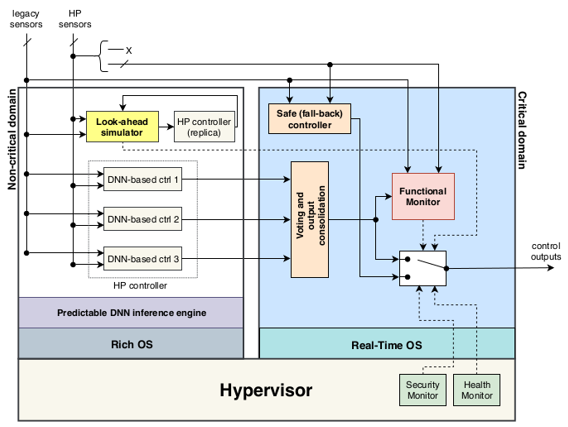
\includegraphics{Figures/figura_35.PNG}
\decoRule
\caption[Arquitectura para redes neuronales artificiales en sistemas críticos]{Arquitectura para redes neuronales artificiales en sistemas críticos \parencite{r5}.}
\label{fig:35}
\end{figure}

\subsection{Consideraciones adicionales de seguridad}
A continuación se presentan algunas consideraciones de seguridad a tener en cuenta al implementar una red neuronal artificial:
\begin{itemize}
    \item \textbf{Datos de entrenamiento confiables:} Para evitar ataques como los del tipo envenenamiento de datos se ha de tener precaución en cuanto al origen de los datos de entrenamiento. Dependiendo de la criticidad en la cual operará el sistema, se podría evaluar generar datos de prueba propios. Si esto no fuese factible, otra opción es chequear los conjunto de datos con algún otro modelo.
    \item \textbf{Restringir accesos al modelo:} El acceso a el modelo de la red neuronal artificial debe estar habilitado solo para personal autorizado, como también la documentación, datos de entrenamiento, parámetros y topología. Solo deben ser expuestas las interfaces de entrada y salida a los demás usuarios.  
    \item \textbf{Resultados específicos:} Si es posible, la salida restringirla sólo al atributo clasificado de forma booleana, sin indicar los porcentajes, para evitar la extracción del modelo.

\end{itemize}
 


\chapter{Experimentos con ataques adversarios} % Main chapter title

\label{Experimentos} % Change X to a consecutive number; for referencing this chapter elsewhere, use \ref{ChapterX}

%----------------------------------------------------------------------------------------
%	SECTION 1
%----------------------------------------------------------------------------------------

En esta sección se presentan distintos experimentos en donde se implementan y evalúan ataques adversarios. Se implementaron en Python desde un notebook generado en Jupyter. También se utilizaron los marcos de trabajos Keras y Tensorflow ejecutando procesos en la GPU a través de CUDA (drivers de tarjeta gráfica Nvidia).


\section{Ambiente de trabajo}
Esta práctica fue realizada en las siguientes condiciones de hardware y software:
\begin{itemize}
    \item Software
        \begin{itemize}
            \item Sistema Operativo: Ubuntu 20.04
            \item nvcc: NVIDIA (R) Cuda compiler driver
            \item Librerías: Keras (Tensorflow como backend)
        \end{itemize}
    \item Hardware
        \begin{itemize}
            \item Procesador: i7-9750H, 2.60 GHz, 6 nucleos, 12 MB Cache
            \item GPU: Nvidia GTX 1650 MAX Q, 4GB
            \item RAM: 32 GB DDR4
        \end{itemize}
\end{itemize}


\section{Repositorio}
El código fuente de estos experimentos se encuentra publicado en Github, y está desarrollado en lenguaje Python, creado en notebooks de Júpiter.
La URL del repositorio es la siguiente:\\ \url{https://github.com/rodrigo-orellana/Seguridad-en-redes-neuronales-artificiales}



\section{Ataques adversarios en fashion MNIST: Transferibilidad}
Este experimento se llevó a cabo con la intención de comprobar la transferibilidad \parencite{r4} de ejemplos adversarios de un modelo a otro cuando ambos modelos poseen el mismo tipo de clasificación. Se diseñó bajo los supuestos siguientes:
\begin{itemize}
    \item El atacante posee acceso solo a ingresar imágenes en la entrada y observar el resultado de la clasificación del modelo objetivo de su ataque.
    \item El atacante tiene acceso al conjunto de datos utilizado en el entrenamiento del modelo objetivo del ataque.
    \item El atacante crea su propio modelo sustituto, en cual posee una arquitectura y parámetros distintos al del modelo objetivo del ataque, pero es entrenado con el mismo conjunto de datos.
    \item El atacante crea ejemplos adversarios utilizando las gradientes descendientes del modelo sustituto y haciendo uso de imágenes de prueba del conjunto de datos.
    \item El atacante ejecuta su ataque con los ejemplos adversarios creados en su modelo sustituto.
\end{itemize}


\subsection{Conjunto de datos fashion MNIST}
Fashion-MNIST es un conjunto de datos de imágenes de los artículos de la tienda de moda Zalando, que consta de un conjunto de entrenamiento de 60.000 ejemplos y un conjunto de validación de 10.000 ejemplos. Cada ejemplo es una imagen en escala de grises de 28x28, asociada con una etiqueta de 10 clases que se muestran en la figura~\ref{fig:36}.

\begin{figure}[!h]
\centering
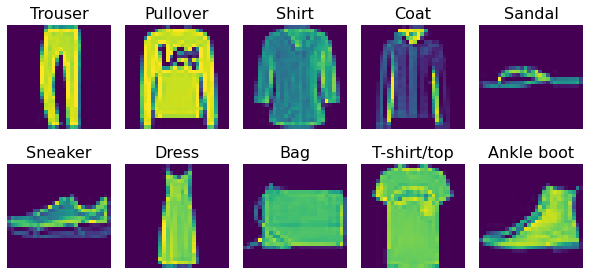
\includegraphics[scale = 0.92]{Figures/figura_36.PNG}
\decoRule
\caption[Redes generativas con adversario (GAN) como defensas]{Muestra de las 10 clases del conjunto de datos fashion-MNIST.}
\label{fig:36}
\end{figure}

\subsection{Modelo sustituto}
Se creó un modelo que llamaremos sustituto, el cual tiene como propósito generar ejemplos adversarios a ser utilizados a otros modelos que presentaremos a continuación en modalidad de caja negra. La red utilizada es una CNN simple, su arquitectura se observa en la figura~\ref{fig:model}.

\begin{figure}[!h]
\centering
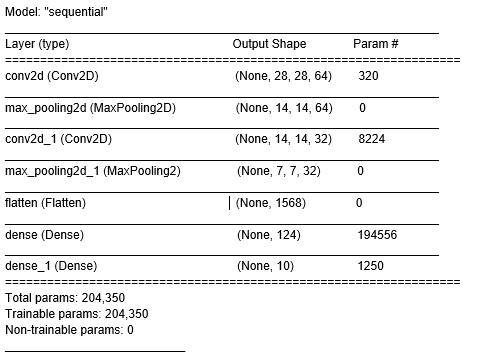
\includegraphics{Figures/model_F_MNIST.PNG}
\decoRule
\caption[Arquitectura modelo sustituto fashion-MNIST]{Arquitectura modelo sustituto}
\label{fig:model}
\end{figure}

Para validar que los modelos creados en el experimento funcionan correctamente presentamos en la figura~\ref{fig:37} una gráfica de exactitud de los modelos validados en los datos de validación. El modelo 01 corresponde al modelo sustituto, mientras que los modelos del 02 al 06 son las víctimas. La exactitud de los modelos varía entre 90\% y 93\%. (95\% es el máximo conocido para este soluciones al conjunto de datos)

\begin{figure}[!h]
\centering
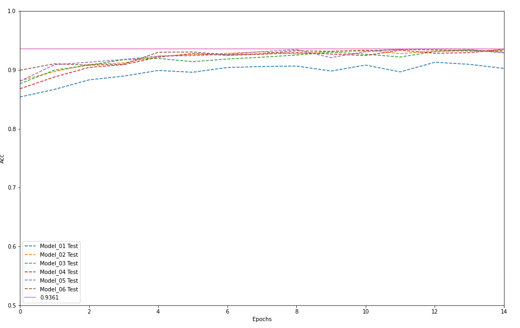
\includegraphics{Figures/figura_37.PNG}
\decoRule
\caption[Arquitectura modelo sustituto fashion-MNIST]{Exactitud de los modelos creados para el experimento.}
\label{fig:37}
\end{figure}

\subsection{Ataque de caja negra}
Se utiliza el conjunto de datos Fashion MNIST y utilizando los cinco modelos CNN víctimas con distintas arquitecturas, los cuales serán atacados. Todos obtuvieron una exactitud mayor al 90\% en los datos de validación. Por otro lado se creó un “modelo sustituto” el cual tiene por objetivo generar ejemplos adversarios utilizando la técnica de FGSM para ser usados en contra de los cinco modelos víctimas. En el modelo sustituto se crean los ejemplos adversarios indicados en las figuras ~\ref{fig:38} y ~\ref{fig:40} con distintos valores de $\varepsilon$. El caso $\varepsilon$= 0 corresponde a la imagen original, mayor a cero es una imagen adversaria. 

\begin{figure}[!h]
\centering
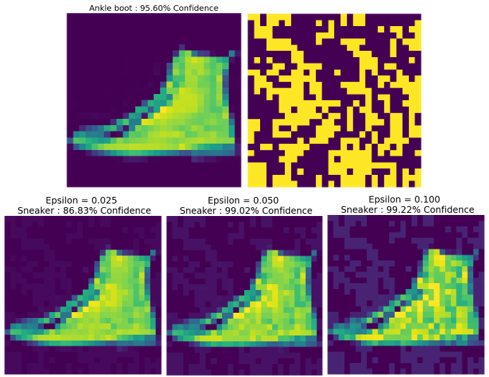
\includegraphics{Figures/figura_38.PNG}
\decoRule
\caption[Ataques adversarios en fashion MNIST.]{Ataques adversarios en fashion MNIST. Fila superior: A la izquierda la imagen original, derecha la matriz de dirección de perturbaciones
Fila inferior: Ejemplos adversarios a partir de distintos valores $\varepsilon$ y su resultado en modelo sustituto.}
\label{fig:38}
\end{figure}


\subsubsection{Preparación ataques adversarios}
Una vez entrenado el modelo sustituto se procedió a la creación del ejemplo adversario. Se implementó la técnica FGSM, en dónde utilizando el marco de trabajo Tensorflow se accedió a la función de gradiente descendiente con la cual pudimos saber donde realizar las modificaciones en la entrada para maximizar el error de clasificación.
Elegimos un par de imágenes de prueba para construir el ejemplo adversario. Se valida la imagen original en el modelo sustituto y este lo clasifica adecuadamente. Se obtiene la matriz de dirección de modificaciones que maximizan el error y luego se definieron distintos valores de $\varepsilon$, parámetro que determina el tamaño de las perturbaciones. 


\subsubsection{Primer ataque: Ankle boot}
En la figura~\ref{fig:38} la fila superior a la izquierda se encuentra la imagen original a utilizada en la creación de los ejemplos adversarios, a su derecha la matriz de dirección de perturbaciones y la fila inferior los ejemplos adversarios generados para distintos valores de $\varepsilon$ según se indica en su cabecera. La imagen original posee una clasificación de “Ankle boot” con un 95,6\% de confianza en el modelo sustituto, lo cual es correcto según su etiqueta. Las imágenes generadas con FGSM fueron clasificadas erróneamente, desde $\varepsilon$= 0.025 con una clasificación distinta en el modelo sustituto.


Ejecutamos el ataque sobre los modelos víctimas, obteniendo los resultados indicados en la figura~\ref{fig:39}. Podemos observar que en el caso de la imagen "Ankle boot" el ataque es 100\% efectivo en el modelo sustituto, éste afectó al 80\% de los modelos víctimas y en donde su ataque es efectivo a partir de un $\varepsilon$=0.1, en donde los modelos lo clasifican como "Coat", "Bag" y "Sneaker".

\begin{figure}[!h]
\centering
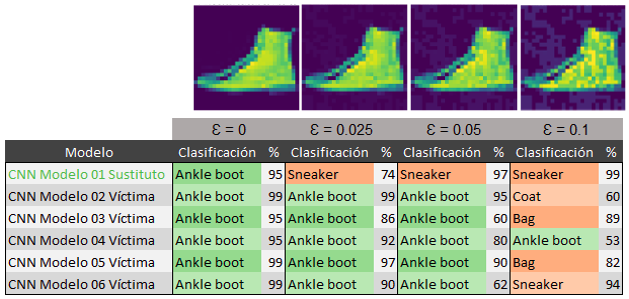
\includegraphics[scale = 0.90]{Figures/figura_39.PNG}
\decoRule
\caption[Resultados ataque 1 con fashion MNIST.]{Resultados ataque con fashion MNIST. En color verde se muestra para cada modelo y cada $\varepsilon$ las clasificaciones correctas. Este ejemplo adversario sólo logró su objetivo con un $\varepsilon$=0.1 en todos los modelos víctimas, a excepción del modelo 4. Fila superior la imagen asociada a cada $\varepsilon$.}
\label{fig:39}
\end{figure}



\subsubsection{Segundo ataque: Coat}
Se elige una segunda imagen del conjunto de datos de validación, cuya etiqueta lo cataloga como “Coat”. Se evalúa en el modelo sustituto y este lo clasifica correctamente con un 80.34\% de confianza, como se muestra en la primera fila, izquierda de la figura~\ref{fig:40}. Luego generamos los ejemplos adversarios de manera similar a como se hizo en el caso anterior con la “Ankle boot” y obtenemos las imágenes de la fila inferior de la figura~\ref{fig:40}.

Ejecutamos el ataque sobre los modelos víctimas, obteniendo los resultados indicados en la figura~\ref{fig:41}. Podemos observar que en el caso de la imagen Coat el ataque es 100\% efectivo en el modelo sustituto, éste afectó al 60\% de los modelos víctimas a partir de un $\varepsilon$=0.025 y luego a partir de un $\varepsilon$=0.05 afecta al 100\%, por lo que este ataque fue más efectivo que el “Ankle boot”, utilizando la misma técnica anterior solo variando la entrada seleccionada para la creación de los ejemplos adversarios.

\begin{figure}[!h]
\centering
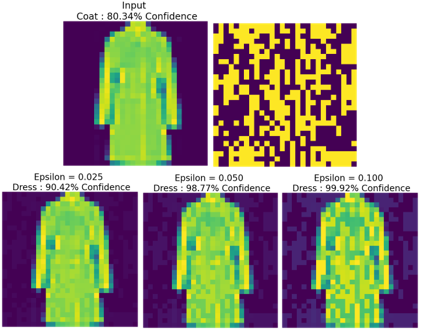
\includegraphics[scale = 1]{Figures/figura_40.PNG}
\decoRule
\caption[Resultados ataque 2 con fashion MNIST.]{Ataque adversario en Fashion MNIST. 
Fila superior: A la izquierda la imagen original, derecha la matriz de dirección de perturbaciones
Fila inferior: Ejemplos adversarios para distintos valores de $\varepsilon$ y su resultado en el modelo sustituto.
}
\label{fig:40}
\end{figure}


\begin{figure}[!h]
\centering
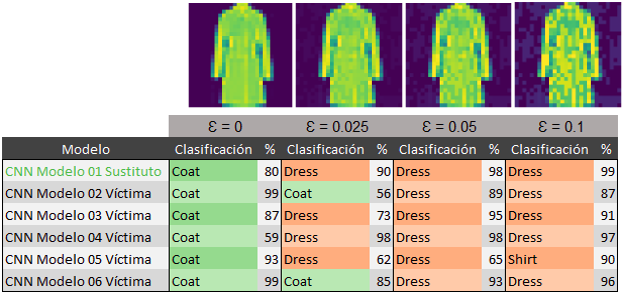
\includegraphics[scale = 0.85]{Figures/figura_41.PNG}
\decoRule
\caption[Resultados ataque 2 con fashion MNIST.]{Resultados ataque con fashion MNIST. En color verde se  muestra  para  cada  modelo  y  cada $\varepsilon$ las  clasificaciones  correctas. Este ejemplo adversario logró su objetivo con un $\varepsilon$=0.05 en todos los modelos víctimas. Fila superior la imagen asociada a cada $\varepsilon$}
\label{fig:41}
\end{figure}


La diferencia entre el primer y segundo ataque indica que la transferibilidad de los ejemplos adversarios depende de la entrada elegida, Por lo que el atacante debería crear varias entradas para su ataque y luego observar cual le servirá para su propósito.

En este experimento cada modelo poseía distintas cantidad de capas, neuronas, funciones de activación, algunas usan drop out y técnicas de aumento del conjunto de entrenamiento, otras no. Se comprueba la propiedad de transferibilidad de ejemplos adversarios generados en un modelo sustituto creado  para atacar a otros modelos a los cuales solo se accede como caja negra.



\subsubsection{Ataque con perturbaciones aleatorias}

Este experimento busca confirmar la efectividad de las técnicas que utilizan el gradiente descendiente para maximizar el error del clasificador de la redes profundas. Para ello realizaremos pruebas en donde se aplicarán perturbaciones a una imagen de entrada, pero en lugar de usar la matriz de dirección de modificaciones que entrega FGSM crearemos un conjunto de matrices con direcciones aleatorias. La figura~\ref{fig:42} muestra las perturbaciones creadas en el experimento, cada una de ellas fue aplicada a una imagen del conjunto de datos de validación para distintos valores de epsilon (tamaño de la perturbación).

En el ataque FGSM realizado sobre el modelo sustituto, cuyos resultados se encuentran en la figura~\ref{fig:39}, fue efectivo desde $\varepsilon$ 0.025. Los resultados del ataque aleatorio se encuentran en el anexo \ref{AppendixA}, en ellos se observa que en las 25 perturbaciones aleatorias, no se logró hacer fallar la clasificación de la misma imagen del modelo sustituto con $\varepsilon$ 0.05 como tampoco con 0.1, luego con 0.2 solo se logró el objetivo del ataque con una de las perturbaciones. Con $\varepsilon$ 0.5 se logró 100\% de efectividad del ataque, pero la imagen resultante no se consideraría un ejemplo adversario, ya que si bien logró el fallo en la clasificación de la imagen, la perturbación es perceptible para el ojo humano. La figura~\ref{fig:43} muestra una comparativa entre la imagen original (a la izquierda) utilizada en el ataque y los resultados de algunas de las perturbaciones aleatorias con  $\varepsilon$= 0.50.


\begin{figure}[!h]
\centering
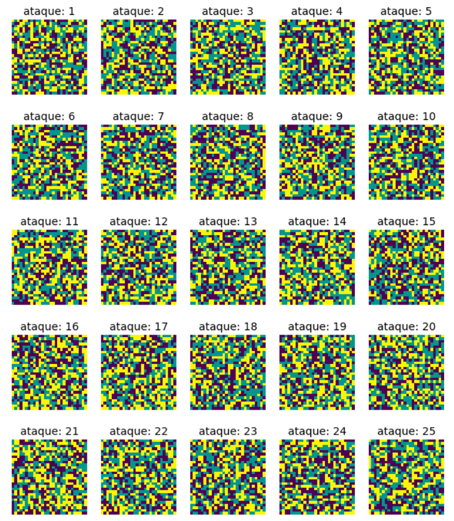
\includegraphics[scale = 1]{Figures/figura_42.PNG}
\decoRule
\caption[Matriz perturbaciones aleatorias aplicadas en el experimento con MNIST.]{Matriz de perturbaciones aleatorias aplicadas en el experimento.}
\label{fig:42}
\end{figure}

\begin{figure}[!h]
\centering
\includegraphics[scale = 0.85]{Figures/figura_43.PNG}
\decoRule
\caption[Matriz perturbaciones aleatorias aplicadas en el experimento con MNIST.]{Comparativa imagen original y perturbación aleatorias con $\varepsilon$=0.5}
\label{fig:43}
\end{figure}

La figura~\ref{fig:44} presenta una comparativa de porcentaje de efectividad de los ataques entre la técnica FGSM versus el ataque aleatorio.

\begin{figure}[!h]
\centering
\includegraphics[scale = 1]{Figures/figura_44.PNG}
\decoRule
\caption[Comparativa de efectividad de los ataques FGSM y aleatorio.]{Comparativa de efectividad de los ataques}
\label{fig:44}
\end{figure}




\section{Ataque adversario en MobileNet V2 e ImageNet}
\subsection{Importación de red pre-entrenada}
Este experimento consistió en generar un ataque a una CNN de clasificación de imágenes con mayor cantidad de detalles, colores y formas, usando para ello un red pre-entrenada. Una red pre-entrenada es una red que fue entrenada previamente en un gran conjunto de datos, típicamente en una tarea de clasificación de imágenes a gran escala y que fue guardada. Esto permite contar con una arquitectura y eficacia ya probada. Por otro lado se atacó un modelo CNN que ha sido ampliamente utilizado, lo cual permitiría que las imágenes construidas para dicho propósito puedan ser utilizadas para atacar otros sistemas donde este se encuentre implementado. El modelo sobre el que se trabajó es el MobileNet V2 \parencite{r58} de la empresa Google. La arquitectura utiliza redes convolutivas con 32 filtros, seguidos de 19 capas residuales de cuello de botella y utiliza ReLU6 como función no lineal. Implementa kernel de tamaño 3x3 como también drop out y normalización durante el entrenamiento. El conjunto de datos utilizado es el ImageNet, el cual es un gran conjunto de datos que consta de imágenes 1.4 millones y 1000 clases cuyo propósito es el uso en investigación \parencite{r59}. 

\subsection{Preparación de ejemplos adversarios}

El conjunto de datos contiene una serie de objetos y animales en sus clases. En este experimento se trabajó con señaléticas de tránsito. La figura~\ref{fig:45}  muestra a las imágenes originales, clasificadas correctamente por el modelo. Estas imágenes no son parte del conjunto de datos, por lo que el modelo generaliza adecuadamente.

\begin{figure}[!h]
\centering
\includegraphics[scale = 1]{Figures/figura_45.PNG}
\decoRule
\caption[Ejemplo MobileNet V2 e ImageNet clasificación imágenes]{MobileNet V2 e ImageNet. Clasificador entrega correcta clasificación a las imágenes originales.}
\label{fig:45}
\end{figure}

Luego se procedió a la creación del ejemplo adversario, utilizando  la técnica de FGSM y las librerías Python 3 de Tensorflow. Con el marco de trabajo Tensorflow se obtiene la matriz de signos de gradientes para cada píxel de las imágenes, la cual indica en qué dirección modificar cada  imagen para maximizar su error en el clasificador (objetivo del ataque). La figura~\ref{fig:46} muestra como se ve dicha matriz al visualizarla como imagen respectivamente para las fotografías antes presentadas.

\begin{figure}[!h]
\centering
\includegraphics[scale = 1]{Figures/figura_46.PNG}
\decoRule
\caption[Ejemplo MobileNet V2 e ImageNet ataque FGSM]{Direcciones de las perturbaciones sugeridas en base a la gradiente descendiente para maximizar error. Izquierda: señalética velocidad máxima, derecha: Cruce peatonal.}
\label{fig:46}
\end{figure}

\subsubsection{Ataque señalética velocidad máxima 40}

Se crearon distintas imágenes, asociadas a distintos valores $\varepsilon$. A menor valor de $\varepsilon$, menos imperceptible el ataque a la vista humana, pero menor probabilidad de que el ataque sea efectivo. A mayor valor, más notable a la vista el ataque, aunque mayor probabilidad de hacer fallar la clasificación. La figura~\ref{fig:47} muestra los resultados de aplicación de perturbaciones para pequeños valores de $\varepsilon$, la primera imagen de la izquierda es la imagen original ($\varepsilon$ igual cero). Hacia la derecha van aumentando los valores de las perturbaciones. Con un pequeño $\varepsilon$=0.01 ya se logró engañar al clasificador, entregando una respuesta distinta a la original y siendo imperceptible la diferencia visual de ambas imágenes. 

\begin{figure}[!h]
\centering
\includegraphics[scale = 0.85]{Figures/figura_47.PNG}
\decoRule
\caption[Perturbaciones FGSM con pequeños $\varepsilon$ señalética velocidad]{Perturbaciones FGSM con pequeños $\varepsilon$.}
\label{fig:47}
\end{figure}

A mayor valores de $\varepsilon$ observamos la notoriedad del ataque a la vista humana, y el modelo lo sigue clasificando erróneamente, como se muestra en la figura~\ref{fig:48}. Como se puede observar, un ataque adversario puede ser ejecutado fácilmente en un modelo importado. Esto permitiría al atacante crear localmente sus imágenes para luego utilizarlas atacando a otros clasificadores creados a partir de la importación del mismo modelo.

\begin{figure}[!h]
\centering
\includegraphics[scale = 0.80]{Figures/figura_48.PNG}
\decoRule
\caption[Perturbaciones FGSM con mayores $\varepsilon$ señalética velocidad]{Perturbaciones FGSM con $\varepsilon$ mayores.}
\label{fig:48}
\end{figure}


\subsubsection{Ataque señalética cruce peatonal}
El segundo ataque a señaléticas entregó similares resultados al anterior como se observa en las figuras~\ref{fig:49} y~\ref{fig:50}. con un pequeño $\varepsilon$=0.01 bastó para hacer fallar la clasificación y el resultado es imperceptible. Se puede observar en la figura~\ref{fig:50} con un $\varepsilon$=0.3 (imagen del centro) la probabilidad asignada a la clasificación errónea es incluso mayor a la entregada a la imagen original.

\begin{figure}[!h]
\centering
\includegraphics[scale = 0.85]{Figures/figura_49.PNG}
\decoRule
\caption[Perturbaciones FGSM con pequeños $\varepsilon$ en cruce peatonal]{Perturbaciones FGSM con pequeños $\varepsilon$.}
\label{fig:49}
\end{figure}

\begin{figure}[!h]
\centering
\includegraphics[scale = 0.83]{Figures/figura_50.PNG}
\decoRule
\caption[Perturbaciones FGSM con mayores $\varepsilon$ en cruce peatonal]{Perturbaciones FGSM con $\varepsilon$ mayores.}
\label{fig:50}
\end{figure}


\section{Ataque adversario placa de matrícula}

Este experimento tiene por propósito demostrar la vulnerabilidad que presentan los sistemas de reconocimiento automático de placas de matrículas de vehículos implementados en redes neuronales. Hoy en día existen varios software y hardware que ofrecen esta funcionalidad, cada día su uso se masifican más. Estos sistemas son utilizados por empresas de parking para controlar los accesos, autopistas para control de velocidad o cobro por uso de tramos, carros policiales para identificación automática de los vehículos que lo anteceden. Su arquitectura en general funciona de manera similar a la presentada en la figura~\ref{fig:51} que fue obtenida de una publicación \parencite{r60}. En la figura se observa que la entrada al sistema es la fotografía de vehículos,  en donde en primer lugar se detecta la presencia de coches, luego se identifica el área en donde se encuentra la matrícula en la imagen. El paso siguiente es rectificar la matrícula mejorando su ángulo, para posteriormente realizar el reconocimiento de los caracteres (OCR: Optical Character Recognition).

\begin{figure}[!h]
\centering
\includegraphics[scale = 0.90]{Figures/figura_51.PNG}
\decoRule
\caption[Flujo de operación de reconocimiento de placas matrículas]{Flujo de operación de reconocimiento de placas matrículas \parencite{r60}.}
\label{fig:51}
\end{figure}

La investigación tomada como referencia \parencite{r60} ofrece además los fuentes de su sistema de detección de matrícula, el cual se utilizó en este estudio como víctima de los ataques, provocando el fallo al clasificar los caracteres de las matrículas que fueron manipuladas.

\subsection{Sistema víctima}
Obtuvimos los fuentes del sistema propuesto en la investigación citada \parencite{r60} la cual divide su funcionamiento en los siguientes pasos:
\begin{enumerate}
    \item Detección de área de la matrícula:
        El sistema implementa un modelo pre-entrenado para la detección y extracción del área de las matrículas, llamado Wpod-Net. Este modelo es capaz de identificar matrículas de 10 países. La figura~\ref{fig:52} muestra los resultados que entrega esta red, enmarcando en rojo las placas matriculas detectadas en cada imagen. .
        
        \begin{figure}[!h]
        \centering
        \includegraphics[scale = 0.9]{Figures/figura_52.PNG}
        \decoRule
        \caption[Detección de placas matrículas]{Detección de área de matrículas \parencite{r60}.}
        \label{fig:52}
        \end{figure}


    \item Identificación de espacio de caracteres:
        El sistema utiliza OpenCV para la segmentación de las áreas donde están ubicados los caracteres de la matrícula, de esta forma se prepara la información para el paso siguiente de reconocimiento de caracteres. La figura~\ref{fig:53} muestra los resultados de este proceso para una matrícula europea.

        \begin{figure}[!h]
        \centering
        \includegraphics[scale = 1]{Figures/figura_53.PNG}
        \decoRule
        \caption[Identificación de espacio de caracteres en placas matrículas]{ Identificación de espacio de caracteres con OpenCV \parencite{r60}.}
        \label{fig:53}
        \end{figure}
    \item OCR [Optical Character Recognition]:
        Una vez detectada la ubicación de cada uno de los caracteres se itera uno a uno pasándolos a la entrada de una red convolutiva que determina su clase, permitiendo obtener la matrícula del coche. La figura~\ref{fig:54} muestra los resultados obtenidos en el artículo citado \parencite{r60}.

         \begin{figure}[!h]
        \centering
        \includegraphics[scale = 0.85]{Figures/figura_54.PNG}
        \decoRule
        \caption[Resultados obtenidos del OCR]{ Resultados obtenidos del OCR \parencite{r60}.}
        \label{fig:54}
        \end{figure}
        
\end{enumerate}

\subsection{Pruebas previas al modelo: Imagen no perturbada}
Se descargó del repositorio Github el proyecto del artículo citado \parencite{r60}. El modelo del clasificado de caracteres posee un exactitud del 97.77\% en cual fue entrenado y validado con el conjunto de datos alfanumérico de 37.623 imágenes que posee 36 clases, aproximadamente 1.000 imágenes por cada caracter. El 10\% se utilizó para validación, y el restante 90\% en entrenamiento. La figura~\ref{fig:58} muestra los resultados del entrenamiento/validación del modelo.

 \begin{figure}[!h]
    \centering
    \includegraphics[scale = 0.85]{Figures/figura_58.PNG}
    \decoRule
    \caption[Resultados del entrenamiento/validación del clasificador de caracteres]{Resultados del entrenamiento/validación del modelo clasificador de caracteres alfanuméricos.}
    \label{fig:58}
\end{figure}



Ejecutamos la prueba con la imagen mostrada en la figura~\ref{fig:55}, observamos la correcta extracción de la matrícula.

 \begin{figure}[!h]
    \centering
    \includegraphics[scale = 1]{Figures/figura_55.PNG}
    \decoRule
    \caption[Pruebas preliminares, extracción de matrícula]{Pruebas preliminares, extracción de matrícula.}
    \label{fig:55}
\end{figure}

Luego continuamos el tratamiento de la imagen para facilitar la posterior lectura de los caracteres, como se muestra en la figura~\ref{fig:56}.

 \begin{figure}[!h]
    \centering
    \includegraphics[scale = 1]{Figures/figura_56.PNG}
    \decoRule
    \caption[Pruebas preliminares, tratamiento de la imagen]{Pruebas preliminares, tratamiento de la imagen.}
    \label{fig:56}
\end{figure}

Posteriormente se identifica las áreas de los caracteres en la imagen como muestra la figura~\ref{fig:57}. Finalmente se procede con el reconocimiento de los caracteres.

 \begin{figure}[!h]
    \centering
    \includegraphics[scale = 0.85]{Figures/figura_57.PNG}
    \decoRule
    \caption[Pruebas preliminares, detección de área de caracteres en la imagen]{Pruebas preliminares, detección de área de caracteres en la imagen.}
    \label{fig:57}
\end{figure}


Los resultados de la clasificación de la imagen original (no perturbada) se encuentran en la figura~\ref{fig:59}, donde observamos que cada caracter fue correctamente identificado. Con esta prueba podemos confirmar que el modelo funciona y podemos comenzar con el ataque.

 \begin{figure}[!h]
    \centering
    \includegraphics[scale = 1]{Figures/figura_59.PNG}
    \decoRule
    \caption[Pruebas preliminares, reconocimiento de los caracteres]{Pruebas preliminares, reconocimiento de los caracteres.}
    \label{fig:59}
\end{figure}

\subsection{Ataque adversario al modelo: Ataque físico}
En este experimento aplicaremos una técnica que simula un ataque físico (mundo real), es decir que simularemos aplicar una especie de parche a una placa matrícula con el objetivo que el clasificador de caracteres falle. Utilizaremos fuerza bruta, modificando un caracter hasta conseguir el objetivo. Se elige atacar utilizando el dígito “1” debido a que en la figura~\ref{fig:22} (ataque Jacobiano a MNIST de dígitos) se puede observar que es el número que menos perturbaciones requiere para hacer fallar al clasificador, por ende el que tiene mayor potencial.
Realizamos pruebas desde menos a más perturbaciones y se logra el objetivo, estableciendo el patrón de perturbación necesario para que el clasificador entregue una salida errónea.
El anexo \ref{AppendixB} muestra las perturbaciones realizadas a una placa matrícula alemana y a una placa matrícula española, de manera manual en un editor de imágenes, en donde se fueron colocando manchas  alrededor del dígito “1”, siguiendo algunas formas obtenidas de la figura~\ref{fig:22}. Se crearon 25 ejemplos adversarios para cada ataque, logrando con 6 obtener fallas en el clasificador en la placa matrícula alemana y 5 en la española.




\subsubsection{Ataque placa matrícula alemana}

La figura~\ref{fig:60} muestra las imágenes que lograron el objetivo del ataque con la placa matrícula alemana. En la interpretación del dígito 1 observamos ocasiones en que fue interpretado como el dígito 3, carácter T y E en el modelo víctima, lo que equivale al 24\% de efectividad del ataque. 

 \begin{figure}[!h]
    \centering
    \includegraphics[scale = 1.1]{Figures/figura_60.PNG}
    \decoRule
    \caption[Ejemplos adversarios placa matrícula alemana]{Ejemplos adversarios que lograron hacer fallar al clasificador placa matrícula alemana.}
    \label{fig:60}
\end{figure}

Para comprobar que el ataque físico es efectivo, se imprimió una fotografía de uno de los ejemplos adversarios (id test 8 de figura~\ref{fig:60}) y luego esta imagen fue fotografiada y pasada nuevamente por el clasificador. La fotografía hizo fallar el modelo entregando el mismo resultado de la imagen modificada digitalmente. La figura~\ref{fig:61} muestra el ejemplo adversario impreso para efectuar el ataque físico, en donde el dígito “1” fue interpretado por un “3”. La alteración de la imagen es levemente perceptible.

 \begin{figure}[!h]
    \centering
    \includegraphics[scale = 1.1]{Figures/figura_61.PNG}
    \decoRule
    \caption[Ejemplo Adversario impreso matrícula alemana]{Ejemplo Adversario impreso. Modelo clasificó dígito “1” cómo “3”. Matrícula alemana.}
    \label{fig:61}
\end{figure}



\subsubsection{Ataque placa matrícula española}
La figura~\ref{fig:62} muestra las imágenes que lograron el objetivo del ataque de la placa matrícula española. Del total de 25 ejemplos adversarios, 5 lograron el fallo del clasificador en la interpretación del primer dígito 1 que posee la matrícula, donde dicho dígito fue interpretado como el carácter T en el modelo víctima. Esto equivale al 20\% de efectividad del ataque. El anexo \ref{AppendixB} posee la totalidad de pruebas realizadas.

 \begin{figure}[!h]
    \centering
    \includegraphics[scale = 1.1]{Figures/figura_62.PNG}
    \decoRule
    \caption[Resultados clasificador con una matrícula española]{Ejemplos adversarios que lograron hacer fallar al clasificador con una matrícula española.}
    \label{fig:62}
\end{figure}




\subsection{Defensa del modelo clasificador matrícula alemana}

Como se observa en los resultados del ataque, fue sencillo hacer fallar el modelo clasificador alfanumérico, esto puede tener relación a que la cantidad de datos de entrenamiento fue insuficiente, en comparación con el conjunto de datos MNIST de dígitos, el cual ofrece hasta 7 veces más imágenes por clase. Por otro lado, se realizan pruebas buscando una arquitectura de la red que ofrezca una robustez mayor frente al ataque. Por lo anterior se observan dos puntos de mejora:



\subsubsection{Defensa 1: Aumento del conjunto de entrenamiento}

El aumento del conjunto de entrenamiento es una técnica que permite aumentar las imágenes de entrenamiento a partir de las existentes, a través de funciones de zoom, rotaciones, desplazamientos, cambios de ángulos perspectivas, inversión vertical y horizontal. Si bien la versión original de la red implementó aumento del conjunto de entrenamiento, esta se modificó para hacerla más efectivo. Los resultados del ataque con la CNN original y la CNN con la nueva configuración se muestran en la figura~\ref{fig:63} en donde se logró reducir la efectividad del ataque del 24\% al 12\%. Entre las diferencias más destacables de esta nueva configuración, es que fue diseñada de acuerdo al formato de las imágenes de entrada, las cuales vienen centradas y sin rotación, por lo que se quitó la utilización de imágenes rotadas que traía el modelo original. Por otro lado se amplió la perspectiva (shear) de manera que generar más diversidad de muestras. El modelo original posee una exactitud del 97.77\%, mientras el modelo con la nueva configuración posee un 97.50\%, una leve disminución, pero a una mayor robustez.

 \begin{figure}[!h]
    \centering
    \includegraphics[scale = 0.85]{Figures/figura_63.PNG}
    \decoRule
    \caption[Resultados defensa 1]{Resultados defensa 1 y modelo original, ajuste al aumento del conjunto de entrenamiento.}
    \label{fig:63}
\end{figure}




\subsubsection{Defensa 2: Función de activación}

En el entrenamiento de redes neuronales se suele poner foco total en la exactitud y la pérdida del clasificador y en base a esto se evalúa si un modelo es bueno o no. En nuestro experimento, el modelo original presenta buenos indicadores, un 97.7\% de exactitud, sin embargo su robustez fue débil frente a unos pocos y simples ataques creados. Se experimentó modificando la arquitectura en búsqueda de mejorar la seguridad de la red frente a un ataque adversario. Estos cambios contemplan modificar cantidad de capas  y de neuronas de la red. La red en análisis es una CNN, de la cual nos enfocamos en cambios sobre las capas posteriores a las convulsiones.
El modelo original presenta a la salida de las convoluciones solo una capa oculta, con una función de activación de tipo RELU con drop out de 0.5 y 128 neuronas. El siguiente experimento consistió en mantener la arquitectura, solo cambiando la función de activación de la capa oculta por una SIGMOID cuya diferencia de observa en la figura~\ref{fig:64}.

 \begin{figure}[!h]
    \centering
    \includegraphics[scale = 1]{Figures/figura_64.PNG}
    \decoRule
    \caption[Función de activación]{Izquierda: Función de activación RELU. Derecha: SIGMOID \parencite{r62}.}
    \label{fig:64}
\end{figure}

Esta función posee mayor linealidad, lo cual podría generar fronteras distintas entre las clases de la red. Se utilizó como base la configuración mejorada de aumento del conjunto de entrenamiento. La exactitud de este nuevo modelo fue levemente mayor al original 97.79\% vs 97.77\%. La efectividad del ataque disminuyó, pasando del modelo original 24\% a  16\%, pero aumentó en un 4\% respecto a la defensa 1. Esto indica que si existe una relación entre la robustez y la función de activación del modelo.




\subsubsection{Defensa 3: Cambio arquitectura}

Se implementa una nueva arquitectura, pasando de una capa oculta a tres, con la siguiente distribución de neuronas en las capas ocultas: 512x512x1024, cada capa con drop out 0.5 y funciones de activación RELU->SIGMOID->SIGMOID. Se utilizó como base la configuración de la defensa 1. Este experimento logró ser totalmente robusto frente al ataque adversario del experimento, llevando la efectividad del ataque a 0\%. En cuanto a la exactitud, esta logró superar levemente a la del modelo original, 97.85\% vs 97.77\%. Esto comprueba la importancia de la arquitectura de un modelo y su estrategia de entrenamiento para brindar robustez frente a ataques.

También se probó con otras arquitecturas las cuales no mejoraron en gran medida la seguridad del modelo. La figura~\ref{fig:65} muestra los distintos resultados de los experimentos de defensa.

 \begin{figure}[!h]
    \centering
    \includegraphics[scale = 0.85]{Figures/figura_65.PNG}
    \decoRule
    \caption[Resultados ataques en distintas arquitecturas. Matrícula alemana]{Resultados ataques en distintas arquitecturas. Matrícula alemana.}
    \label{fig:65}
\end{figure}




\subsection{Defensa del modelo clasificador matrícula española}

Se aplicó la mejor contramedida formulada para el ataque a la matrícula alemana para la defensa de la matrícula española, logrando replicar el resultado. La figura~\ref{fig:66} muestra los resultados en donde observamos que aplicando los cambios en el modelo señalado como “CNN Defensa 03” se logra evadir el 100\% de los ataques creados.
\begin{figure}[!h]
    \centering
    \includegraphics[scale = 0.85]{Figures/figura_66.PNG}
    \decoRule
    \caption[Resultados ataques en distintas arquitecturas. Matrícula española]{Resultados ataques en distintas arquitecturas. Matrícula española.}
    \label{fig:66}
\end{figure} 


\chapter{Conclusiones} % Main chapter title

\label{Conclusiones} % Change X to a consecutive number; for referencing this chapter elsewhere, use \ref{ChapterX}

%----------------------------------------------------------------------------------------
%	SECTION 1
%----------------------------------------------------------------------------------------
En este trabajo se ha presentado un estado del arte en temas de seguridad en redes neuronales artificiales, que como se muestra en el documento, es un tema que ha tomado gran interés científico en los últimos años. Se han estudiado, citado y relacionado diversas investigaciones que muestran las vulnerabilidades que presentan los sistemas de inteligencia artificial, con particular énfasis en la sensibilidad de los modelos de clasificación al ser atacadas con pequeñas perturbaciones en sus entradas, las que incluso pueden ser imperceptibles a la revisión humana. También se presentaron técnicas que intentan dar robustez a los modelos frente a dichos ataques, pero estas solo brindan una protección parcial para ciertos tipos de ataques particulares. La seguridad en las redes neuronales es un tema abierto al día de hoy y diversos equipos de investigación se encuentran trabajando en la búsqueda de una solución que garantice dicha seguridad, pero también se siguen descubriendo nuevas técnicas de ataques.

En los experimentos realizados se pudo observar que ciertos modelos fueron fácilmente vulnerados. Se logró perpetuar un ataque de caja blanca en un modelo propio, como también en un modelo importado pre-entrenado con una compleja arquitectura y ampliamente usado, haciendo uso la función de gradiente descendiente de optimización de la red de manera invertida. Luego se demostró que las entradas generadas para el ataque pueden ser utilizadas para efectuar nuevos ataques a otros modelos que implementan el mismo tipo de clasificación, pero distintas arquitecturas, debido a una estudiada característica de las redes neuronales profundas llamadas transferibilidad en ataques de caja negra. Luego utilizando los mismos conjuntos de datos, se realizó una comparativa de los resultados de un ataque utilizando una de las técnicas presentadas en el documento y un ataque con manipulación aleatoria, demostrando la efectividad del primero.

También se realizaron experimentos usando imágenes de señaléticas de tránsito para resaltar los peligros que conlleva el uso de esta tecnología en las aplicaciones de conducción automática de vehículos, aportando además estudios que detallan sus riesgos, como también noticias recientes de incidentes relacionados a esta tecnología. Las imágenes manipuladas para el ataque presentan perturbaciones imperceptibles a la vista humana, pero de gran impacto en el resultado del clasificador de la red neuronal profunda.

En otro experimento realizado en este estudio, se usó como víctima de ataque un sistema que utilizando una red de aprendizaje profundo, detecta e interpreta placas matrículas de vehículos. Esta fue obtenida de una investigación publicada en el año 2018. Sobre este sistema se ejecutó un ataque físico de caja negra, manipulando imágenes con pequeñas manchas situadas de manera aleatoria para hacer fallar la interpretación de los dígitos en la matrícula de entrada. Se trabajó con 2 placas matrículas obteniendo en ambas un porcentaje de efectividad en los ataques de 24\% en el primer experimento y 20\% en el segundo. Luego se demostró que el modelo era perfectible en cuanto a su robustez, tanto en la técnica de entrenamiento como en su arquitectura, logrando generar un nuevo modelo clasificador el cual resultó ser robusto en un 100\% a estos ataques formulados en el experimento. Esto demostró la existencia de una relación entre la robustez de un modelo y su arquitectura, como también la importancia de contar con una cantidad amplia de datos de entrenamientos aun cuando las pruebas de efectividad del modelo sean satisfactorias.




\chapter{Trabajo futuro} % Main chapter title

\label{Futuro} % Change X to a consecutive number; for referencing this chapter elsewhere, use \ref{ChapterX}

%----------------------------------------------------------------------------------------
%	SECTION 1
%----------------------------------------------------------------------------------------


Una vez que se han descrito los resultados más relevantes que se han obtenido durante la realización de este trabajo, se sugiere una serie de puntos de líneas de continuidad para investigaciones futuras:
\begin{itemize}
    \item El estudio de nuevas técnicas de ataques físicos (mundo real) a sistemas de visión artificial basados en redes neuronales artificiales, utilizando algoritmos genéticos para identificar la ubicación que maximiza el error del clasificador en la distribución de las perturbaciones. Podría recibir como parámetro la imagen víctima y la forma de las pegatinas a disponer (rectangular, redonda), cantidad y tamaño.  
    \item Creación de una nueva metodología en la identificación de dígitos de placas matrículas con redes neuronales artificiales de manera robusta, filtrando las perturbaciones provenientes de ataques. Este podría corregir formas no habituales en dígitos previamente conocidos en cuanto a las proporciones de cada uno de ellos, de modo de maximizar la eficacia de su resultado.
    \item Generación de un nuevo marco de trabajo evaluador de robustez de modelos de visión artificial basados en redes neuronales artificiales. Este podría estudiar las fronteras de clasificación generadas y además a través de ataques éticos establecer el nivel de seguridad que posee el modelo analizado, con el fin de proporcionar al arquitecto de la red un indicador sobre el nivel de robustez que posee el modelo. Este podría establecer una métrica para esta característica que permita comparaciones%.\parencite{r5}
    
\end{itemize}








%----------------------------------------------------------------------------------------
%	THESIS CONTENT - APPENDICES
%----------------------------------------------------------------------------------------

\appendix % Cue to tell LaTeX that the following "chapters" are Appendices

% Include the appendices of the thesis as separate files from the Appendices folder
% Uncomment the lines as you write the Appendices

% Appendix A

\renewcommand{\appendixname}{Anexo}
\chapter{Ataque con perturbaciones aleatorias FASHION MNIST. 
} % Main appendix title

\label{AppendixA} % For referencing this appendix elsewhere, use \ref{AppendixA}

Ejemplos adversarios de ataque con perturbaciones aleatorias a un modelo CNN, clasificador del conjunto de datos FASHION MNIST, con epsilon (magnitud de perturbación) 0.05, 0.1, 0.2 y 0.5. En rojo los ataques efectivos. Las imágenes generadas con epsilon 0.5 no serían consideradas como  ejemplos adversarios, ya que la perturbación es perceptible a la vista humana.
\begin{figure}[!h]
    \centering
    \includegraphics[scale = 0.85]{Figures/figura_67_1.PNG}
    \label{fig:67_1}
\end{figure}

\begin{figure}[!h]
    \centering
    \includegraphics[scale = 0.85]{Figures/figura_67_2.PNG}
    \label{fig:67_2}
\end{figure}

\begin{figure}[!h]
    \centering
    \includegraphics[scale = 0.85]{Figures/figura_67_3.PNG}
    \label{fig:67_3}
\end{figure}

\begin{figure}[!h]
    \centering
    \includegraphics[scale = 0.85]{Figures/figura_67_4.PNG}
    \label{fig:67_4}
\end{figure}

\begin{figure}[!h]
    \centering
    \includegraphics[scale = 0.85]{Figures/figura_67_5.PNG}
    \decoRule
    \caption[Ataque con perturbaciones aleatorias]{Ataque con perturbaciones aleatorias a modelo clasificador del conjunto de datos de FASHION MNIST.}
    \label{fig:6_5}
\end{figure}
% Appendix B

\renewcommand{\appendixname}{Anexo}
\chapter{Ataque físico placas matrículas} % Main appendix title

\label{AppendixB} % For referencing this appendix elsewhere, use \ref{AppendixA}
\section{Placa matrícula alemana}
Ejemplos adversarios físicos de ataque de fuerza bruta para confundir la interpretación del dígito 1 en modelo Wpod-Net [60] con placa matrícula alemana.

\begin{figure}[!h]
    \centering
    \includegraphics[scale = 0.85]{Figures/figura_68_1.PNG}
    \label{fig:68_1}
\end{figure}

\begin{figure}[!h]
    \centering
    \includegraphics[scale = 0.85]{Figures/figura_68_2.PNG}
    \decoRule
    \caption[Ejemplos adversarios creados por fuerza bruta. placa matrícula alemana.
]{Ejemplos adversarios creados por fuerza bruta. placa matrícula alemana.}
    \label{fig:68_2}
\end{figure}


\section{Placa matrícula española}
Ejemplos adversarios físicos de ataque de fuerza bruta para confundir la interpretación del dígito 1 en modelo Wpod-Net [60] con placa matrícula española.

\begin{figure}[!h]
    \centering
    \includegraphics[scale = 0.85]{Figures/figura_69_1.PNG}
    \label{fig:69_1}
\end{figure}

\begin{figure}[!h]
    \centering
    \includegraphics[scale = 0.85]{Figures/figura_69_2.PNG}
    \decoRule
    \caption[Ejemplos adversarios creados por fuerza bruta. placa matrícula española.]{Ejemplos adversarios creados por fuerza bruta. placa matrícula española.}
    \label{fig:69_2}
\end{figure}
%% Appendix: Declaration of Originality

\chapter{Declaration of Originality} % Main appendix title

\label{DeclarationOfOriginalityZHAW} % For referencing this appendix elsewhere, use \ref{AppendixA}

\includepdf[pages=-]{Appendices/plagiatserklaerung-master-eng.pdf}
 % from https://www.zhaw.ch/en/lsfm/study/studiweb/master-ls/masters-thesis/
%% Appendix B

\renewcommand{\appendixname}{Anexo}
\chapter{Ataque físico placas matrículas} % Main appendix title

\label{AppendixB} % For referencing this appendix elsewhere, use \ref{AppendixA}
\section{Placa matrícula alemana}
Ejemplos adversarios físicos de ataque de fuerza bruta para confundir la interpretación del dígito 1 en modelo Wpod-Net [60] con placa matrícula alemana.

\begin{figure}[!h]
    \centering
    \includegraphics[scale = 0.85]{Figures/figura_68_1.PNG}
    \label{fig:68_1}
\end{figure}

\begin{figure}[!h]
    \centering
    \includegraphics[scale = 0.85]{Figures/figura_68_2.PNG}
    \decoRule
    \caption[Ejemplos adversarios creados por fuerza bruta. placa matrícula alemana.
]{Ejemplos adversarios creados por fuerza bruta. placa matrícula alemana.}
    \label{fig:68_2}
\end{figure}


\section{Placa matrícula española}
Ejemplos adversarios físicos de ataque de fuerza bruta para confundir la interpretación del dígito 1 en modelo Wpod-Net [60] con placa matrícula española.

\begin{figure}[!h]
    \centering
    \includegraphics[scale = 0.85]{Figures/figura_69_1.PNG}
    \label{fig:69_1}
\end{figure}

\begin{figure}[!h]
    \centering
    \includegraphics[scale = 0.85]{Figures/figura_69_2.PNG}
    \decoRule
    \caption[Ejemplos adversarios creados por fuerza bruta. placa matrícula española.]{Ejemplos adversarios creados por fuerza bruta. placa matrícula española.}
    \label{fig:69_2}
\end{figure}
%\include{Appendices/AppendixC}




%----------------------------------------------------------------------------------------
%	BIBLIOGRAPHY
%----------------------------------------------------------------------------------------
%\bibliographystyle{acm}
\printbibliography[heading=bibintoc]

%----------------------------------------------------------------------------------------




\end{document}  
